\documentclass[twoside]{book}

% Packages required by doxygen
\usepackage{calc}
\usepackage{doxygen}
\usepackage{graphicx}
\usepackage[utf8]{inputenc}
\usepackage{makeidx}
\usepackage{multicol}
\usepackage{multirow}
\usepackage{textcomp}
\usepackage[table]{xcolor}

% Font selection
\usepackage[T1]{fontenc}
\usepackage{mathptmx}
\usepackage[scaled=.90]{helvet}
\usepackage{courier}
\usepackage{amssymb}
\usepackage{sectsty}
\renewcommand{\familydefault}{\sfdefault}
\allsectionsfont{%
  \fontseries{bc}\selectfont%
  \color{darkgray}%
}
\renewcommand{\DoxyLabelFont}{%
  \fontseries{bc}\selectfont%
  \color{darkgray}%
}

% Page & text layout
\usepackage{geometry}
\geometry{%
  a4paper,%
  top=2.5cm,%
  bottom=2.5cm,%
  left=2.5cm,%
  right=2.5cm%
}
\tolerance=750
\hfuzz=15pt
\hbadness=750
\setlength{\emergencystretch}{15pt}
\setlength{\parindent}{0cm}
\setlength{\parskip}{0.2cm}
\makeatletter
\renewcommand{\paragraph}{%
  \@startsection{paragraph}{4}{0ex}{-1.0ex}{1.0ex}{%
    \normalfont\normalsize\bfseries\SS@parafont%
  }%
}
\renewcommand{\subparagraph}{%
  \@startsection{subparagraph}{5}{0ex}{-1.0ex}{1.0ex}{%
    \normalfont\normalsize\bfseries\SS@subparafont%
  }%
}
\makeatother

% Headers & footers
\usepackage{fancyhdr}
\pagestyle{fancyplain}
\fancyhead[LE]{\fancyplain{}{\bfseries\thepage}}
\fancyhead[CE]{\fancyplain{}{}}
\fancyhead[RE]{\fancyplain{}{\bfseries\leftmark}}
\fancyhead[LO]{\fancyplain{}{\bfseries\rightmark}}
\fancyhead[CO]{\fancyplain{}{}}
\fancyhead[RO]{\fancyplain{}{\bfseries\thepage}}
\fancyfoot[LE]{\fancyplain{}{}}
\fancyfoot[CE]{\fancyplain{}{}}
\fancyfoot[RE]{\fancyplain{}{\bfseries\scriptsize Generated on Mon Feb 17 2014 18:48:22 for Movies2HDD by Doxygen }}
\fancyfoot[LO]{\fancyplain{}{\bfseries\scriptsize Generated on Mon Feb 17 2014 18:48:22 for Movies2HDD by Doxygen }}
\fancyfoot[CO]{\fancyplain{}{}}
\fancyfoot[RO]{\fancyplain{}{}}
\renewcommand{\footrulewidth}{0.4pt}
\renewcommand{\chaptermark}[1]{%
  \markboth{#1}{}%
}
\renewcommand{\sectionmark}[1]{%
  \markright{\thesection\ #1}%
}

% Indices & bibliography
\usepackage{natbib}
\usepackage[titles]{tocloft}
\setcounter{tocdepth}{3}
\setcounter{secnumdepth}{5}
\makeindex

% Hyperlinks (required, but should be loaded last)
\usepackage{ifpdf}
\ifpdf
  \usepackage[pdftex,pagebackref=true]{hyperref}
\else
  \usepackage[ps2pdf,pagebackref=true]{hyperref}
\fi
\hypersetup{%
  colorlinks=true,%
  linkcolor=blue,%
  citecolor=blue,%
  unicode%
}

% Custom commands
\newcommand{\clearemptydoublepage}{%
  \newpage{\pagestyle{empty}\cleardoublepage}%
}


%===== C O N T E N T S =====

\begin{document}

% Titlepage & ToC
\hypersetup{pageanchor=false}
\pagenumbering{roman}
\begin{titlepage}
\vspace*{7cm}
\begin{center}%
{\Large Movies2\-H\-D\-D }\\
\vspace*{1cm}
{\large Generated by Doxygen 1.8.4}\\
\vspace*{0.5cm}
{\small Mon Feb 17 2014 18:48:22}\\
\end{center}
\end{titlepage}
\clearemptydoublepage
\tableofcontents
\clearemptydoublepage
\pagenumbering{arabic}
\hypersetup{pageanchor=true}

%--- Begin generated contents ---
\chapter{movies2hdd}
\label{md_README}
\hypertarget{md_README}{}
A simple set of python scripts and libraries to work with movies. I use it with my Dream\-Box.
\begin{DoxyItemize}
\item Homepage\-: \href{http://elchi.github.io/movies2hdd}{\tt http\-://elchi.\-github.\-io/movies2hdd} (It is empty.)
\item Documentation of the A\-P\-I\-: \href{http://elchi.github.io/movies2hdd/docs/html/}{\tt http\-://elchi.\-github.\-io/movies2hdd/docs/html/} (generated using doxygen) 


\end{DoxyItemize}

Why should I use it?
\begin{DoxyItemize}
\item It is written entirely in Python.
\item It supports both 2.\-7 {\itshape and} 3 {\itshape at the same time}. (!)
\item It is a class.
\item It is not finished. 


\end{DoxyItemize}

Features\-:
\begin{DoxyItemize}
\item a C\-L\-I
\begin{DoxyItemize}
\item a line-\/based interface
\item a G\-U\-I
\item a simple movie converter (.ts to .mpg, will delete additional audio tracks!)
\end{DoxyItemize}
\item a library
\begin{DoxyItemize}
\item connects to a Dream\-Box via F\-T\-P
\item searches for movies
\item downloads movies
\item filters meta data
\item queries thetvdb.\-com
\item converts the movies 
\end{DoxyItemize}
\end{DoxyItemize}
\chapter{Namespace Index}
\section{Namespace List}
Here is a list of all namespaces with brief descriptions\-:\begin{DoxyCompactList}
\item\contentsline{section}{\hyperlink{namespacemovies2hdd}{movies2hdd} }{\pageref{namespacemovies2hdd}}{}
\item\contentsline{section}{\hyperlink{namespacemovies2hdd_1_1convert}{movies2hdd.\-convert} }{\pageref{namespacemovies2hdd_1_1convert}}{}
\item\contentsline{section}{\hyperlink{namespacemovies2hdd_1_1gui}{movies2hdd.\-gui} }{\pageref{namespacemovies2hdd_1_1gui}}{}
\item\contentsline{section}{\hyperlink{namespacemovies2hdd_1_1lbi}{movies2hdd.\-lbi} }{\pageref{namespacemovies2hdd_1_1lbi}}{}
\end{DoxyCompactList}

\chapter{Hierarchical Index}
\section{Class Hierarchy}
This inheritance list is sorted roughly, but not completely, alphabetically\-:\begin{DoxyCompactList}
\item \contentsline{section}{movies2hdd.\-Movies2\-H\-D\-D}{\pageref{classmovies2hdd_1_1_movies2_h_d_d}}{}
\item Q\-Dialog\begin{DoxyCompactList}
\item \contentsline{section}{movies2hdd.\-gui.\-Series\-Selection}{\pageref{classmovies2hdd_1_1gui_1_1_series_selection}}{}
\end{DoxyCompactList}
\item Q\-Wizard\-Page\begin{DoxyCompactList}
\item \contentsline{section}{movies2hdd.\-gui.\-Step1}{\pageref{classmovies2hdd_1_1gui_1_1_step1}}{}
\item \contentsline{section}{movies2hdd.\-gui.\-Step2}{\pageref{classmovies2hdd_1_1gui_1_1_step2}}{}
\item \contentsline{section}{movies2hdd.\-gui.\-Step3}{\pageref{classmovies2hdd_1_1gui_1_1_step3}}{}
\end{DoxyCompactList}
\end{DoxyCompactList}

\chapter{Class Index}
\section{Class List}
Here are the classes, structs, unions and interfaces with brief descriptions\-:\begin{DoxyCompactList}
\item\contentsline{section}{\hyperlink{classmovies2hdd_1_1gui_1_1_main_window}{movies2hdd.\-gui.\-Main\-Window} }{\pageref{classmovies2hdd_1_1gui_1_1_main_window}}{}
\item\contentsline{section}{\hyperlink{classmovies2hdd_1_1_movies2_h_d_d}{movies2hdd.\-Movies2\-H\-D\-D} }{\pageref{classmovies2hdd_1_1_movies2_h_d_d}}{}
\end{DoxyCompactList}

\chapter{File Index}
\section{File List}
Here is a list of all files with brief descriptions\-:\begin{DoxyCompactList}
\item\contentsline{section}{\hyperlink{cli_8py}{cli.\-py} }{\pageref{cli_8py}}{}
\item\contentsline{section}{\hyperlink{convert_movie_8py}{convert\-Movie.\-py} }{\pageref{convert_movie_8py}}{}
\item\contentsline{section}{\hyperlink{movies2hdd_8py}{movies2hdd.\-py} }{\pageref{movies2hdd_8py}}{}
\end{DoxyCompactList}

\chapter{Namespace Documentation}
\hypertarget{namespacemovies2hdd}{\section{movies2hdd Namespace Reference}
\label{namespacemovies2hdd}\index{movies2hdd@{movies2hdd}}
}
\subsection*{Namespaces}
\begin{DoxyCompactItemize}
\item 
\hyperlink{namespacemovies2hdd_1_1convert}{convert}
\item 
\hyperlink{namespacemovies2hdd_1_1gui}{gui}
\item 
\hyperlink{namespacemovies2hdd_1_1lbi}{lbi}
\end{DoxyCompactItemize}
\subsection*{Classes}
\begin{DoxyCompactItemize}
\item 
class \hyperlink{classmovies2hdd_1_1_movies2_h_d_d}{Movies2\-H\-D\-D}
\end{DoxyCompactItemize}

\hypertarget{namespacemovies2hdd_1_1convert}{\section{movies2hdd.\-convert Namespace Reference}
\label{namespacemovies2hdd_1_1convert}\index{movies2hdd.\-convert@{movies2hdd.\-convert}}
}
\subsection*{Variables}
\begin{DoxyCompactItemize}
\item 
list \hyperlink{namespacemovies2hdd_1_1convert_aa56ab068434359bf27101c2903a2a076}{movie} = sys.\-argv\mbox{[}1\mbox{]}
\end{DoxyCompactItemize}


\subsection{Variable Documentation}
\hypertarget{namespacemovies2hdd_1_1convert_aa56ab068434359bf27101c2903a2a076}{\index{movies2hdd\-::convert@{movies2hdd\-::convert}!movie@{movie}}
\index{movie@{movie}!movies2hdd::convert@{movies2hdd\-::convert}}
\subsubsection[{movie}]{\setlength{\rightskip}{0pt plus 5cm}tuple movies2hdd.\-convert.\-movie = sys.\-argv\mbox{[}1\mbox{]}}}\label{namespacemovies2hdd_1_1convert_aa56ab068434359bf27101c2903a2a076}


Definition at line 19 of file convert.\-py.


\hypertarget{namespacemovies2hdd_1_1gui}{\section{movies2hdd.\-gui Namespace Reference}
\label{namespacemovies2hdd_1_1gui}\index{movies2hdd.\-gui@{movies2hdd.\-gui}}
}
\subsection*{Classes}
\begin{DoxyCompactItemize}
\item 
class \hyperlink{classmovies2hdd_1_1gui_1_1_main_window}{Main\-Window}
\end{DoxyCompactItemize}
\subsection*{Variables}
\begin{DoxyCompactItemize}
\item 
tuple \hyperlink{namespacemovies2hdd_1_1gui_a5113ba41da39d51855bd15d8cf47d7be}{app} = Py\-Side.\-Qt\-Gui.\-Q\-Application(sys.\-argv)
\item 
tuple \hyperlink{namespacemovies2hdd_1_1gui_a47850301e02e470855a027b38dd4b229}{Movies2\-H\-D\-D} = \hyperlink{classmovies2hdd_1_1_movies2_h_d_d}{movies2hdd.\-Movies2\-H\-D\-D}()
\item 
tuple \hyperlink{namespacemovies2hdd_1_1gui_ab66ae08952e6997fa86b05e376de756a}{mainwindow} = \hyperlink{classmovies2hdd_1_1gui_1_1_main_window}{Main\-Window}()
\end{DoxyCompactItemize}


\subsection{Variable Documentation}
\hypertarget{namespacemovies2hdd_1_1gui_a5113ba41da39d51855bd15d8cf47d7be}{\index{movies2hdd\-::gui@{movies2hdd\-::gui}!app@{app}}
\index{app@{app}!movies2hdd::gui@{movies2hdd\-::gui}}
\subsubsection[{app}]{\setlength{\rightskip}{0pt plus 5cm}tuple movies2hdd.\-gui.\-app = Py\-Side.\-Qt\-Gui.\-Q\-Application(sys.\-argv)}}\label{namespacemovies2hdd_1_1gui_a5113ba41da39d51855bd15d8cf47d7be}


Definition at line 34 of file gui.\-py.

\hypertarget{namespacemovies2hdd_1_1gui_ab66ae08952e6997fa86b05e376de756a}{\index{movies2hdd\-::gui@{movies2hdd\-::gui}!mainwindow@{mainwindow}}
\index{mainwindow@{mainwindow}!movies2hdd::gui@{movies2hdd\-::gui}}
\subsubsection[{mainwindow}]{\setlength{\rightskip}{0pt plus 5cm}tuple movies2hdd.\-gui.\-mainwindow = {\bf Main\-Window}()}}\label{namespacemovies2hdd_1_1gui_ab66ae08952e6997fa86b05e376de756a}


Definition at line 77 of file gui.\-py.

\hypertarget{namespacemovies2hdd_1_1gui_a47850301e02e470855a027b38dd4b229}{\index{movies2hdd\-::gui@{movies2hdd\-::gui}!Movies2\-H\-D\-D@{Movies2\-H\-D\-D}}
\index{Movies2\-H\-D\-D@{Movies2\-H\-D\-D}!movies2hdd::gui@{movies2hdd\-::gui}}
\subsubsection[{Movies2\-H\-D\-D}]{\setlength{\rightskip}{0pt plus 5cm}tuple movies2hdd.\-gui.\-Movies2\-H\-D\-D = {\bf movies2hdd.\-Movies2\-H\-D\-D}()}}\label{namespacemovies2hdd_1_1gui_a47850301e02e470855a027b38dd4b229}


Definition at line 38 of file gui.\-py.


\hypertarget{namespacemovies2hdd_1_1lbi}{\section{movies2hdd.\-lbi Namespace Reference}
\label{namespacemovies2hdd_1_1lbi}\index{movies2hdd.\-lbi@{movies2hdd.\-lbi}}
}
\subsection*{Functions}
\begin{DoxyCompactItemize}
\item 
def \hyperlink{namespacemovies2hdd_1_1lbi_aa411fd2536c5b5990b10eefa5013632a}{connect}
\item 
def \hyperlink{namespacemovies2hdd_1_1lbi_af95b673a57b5470449d62aaf07b91cde}{disconnect}
\item 
def \hyperlink{namespacemovies2hdd_1_1lbi_a8a952cc0a80b1f4ab0bb4d1eaf8f1cfd}{search}
\item 
def \hyperlink{namespacemovies2hdd_1_1lbi_a68a02cd4a9f9c827984c06b24947f42a}{select}
\item 
def \hyperlink{namespacemovies2hdd_1_1lbi_a7cffc384bf2cf29f12ea83b2c59800d0}{save}
\item 
def \hyperlink{namespacemovies2hdd_1_1lbi_a613308653e921ffefd9d15bd912d45f6}{download}
\item 
def \hyperlink{namespacemovies2hdd_1_1lbi_a575a370ef89b527cbda766ff0341e3b4}{rename}
\item 
def \hyperlink{namespacemovies2hdd_1_1lbi_af82814dc0312f2a2a8de4672e6f79c6e}{convert}
\item 
def \hyperlink{namespacemovies2hdd_1_1lbi_a57f4964811a71e55d727484d464ea6e2}{quit}
\end{DoxyCompactItemize}
\subsection*{Variables}
\begin{DoxyCompactItemize}
\item 
tuple \hyperlink{namespacemovies2hdd_1_1lbi_a0a37f11b0348a8fcc9af17541471fbd8}{Movies2\-H\-D\-D} = \hyperlink{classmovies2hdd_1_1_movies2_h_d_d}{movies2hdd.\-Movies2\-H\-D\-D}()
\item 
\hyperlink{namespacemovies2hdd_1_1lbi_a4bc534737690c0a51a760418d39e3753}{ask} = raw\-\_\-input
\item 
tuple \hyperlink{namespacemovies2hdd_1_1lbi_ab0bb9564b6047c61086071bdae2ba4ce}{answer} = int(\hyperlink{namespacemovies2hdd_1_1lbi_a4bc534737690c0a51a760418d39e3753}{ask}(\char`\"{}$>$ \char`\"{}))
\end{DoxyCompactItemize}


\subsection{Function Documentation}
\hypertarget{namespacemovies2hdd_1_1lbi_aa411fd2536c5b5990b10eefa5013632a}{\index{movies2hdd\-::lbi@{movies2hdd\-::lbi}!connect@{connect}}
\index{connect@{connect}!movies2hdd::lbi@{movies2hdd\-::lbi}}
\subsubsection[{connect}]{\setlength{\rightskip}{0pt plus 5cm}def movies2hdd.\-lbi.\-connect (
\begin{DoxyParamCaption}
{}
\end{DoxyParamCaption}
)}}\label{namespacemovies2hdd_1_1lbi_aa411fd2536c5b5990b10eefa5013632a}


Definition at line 26 of file lbi.\-py.


\begin{DoxyCode}
26 
27 \textcolor{keyword}{def }\hyperlink{namespacemovies2hdd_1_1lbi_aa411fd2536c5b5990b10eefa5013632a}{connect}():
28     \textcolor{keywordflow}{print} (\textcolor{stringliteral}{"Connect to your DreamBox"})
29     host = \hyperlink{namespacemovies2hdd_1_1lbi_a4bc534737690c0a51a760418d39e3753}{ask}(\textcolor{stringliteral}{"Host: "})
30     user = \hyperlink{namespacemovies2hdd_1_1lbi_a4bc534737690c0a51a760418d39e3753}{ask}(\textcolor{stringliteral}{"User: "})
31     \textcolor{keywordflow}{print} (\textcolor{stringliteral}{"Your password will be sent unencryptedly!!!"})
32     \textcolor{keywordflow}{print} (\textcolor{stringliteral}{"Don't do this if you don't trust this network."})
33     \textcolor{keywordflow}{print} (\textcolor{stringliteral}{"Otherwise, please tunnel this connection via SSH."})
34     pwd = getpass(\textcolor{stringliteral}{"Password: "})
35     \textcolor{keywordflow}{print} (\textcolor{stringliteral}{"Connecting..."})
36     Movies2HDD.connect(host, user, pwd)
\textcolor{comment}{#}
\end{DoxyCode}
\hypertarget{namespacemovies2hdd_1_1lbi_af82814dc0312f2a2a8de4672e6f79c6e}{\index{movies2hdd\-::lbi@{movies2hdd\-::lbi}!convert@{convert}}
\index{convert@{convert}!movies2hdd::lbi@{movies2hdd\-::lbi}}
\subsubsection[{convert}]{\setlength{\rightskip}{0pt plus 5cm}def movies2hdd.\-lbi.\-convert (
\begin{DoxyParamCaption}
{}
\end{DoxyParamCaption}
)}}\label{namespacemovies2hdd_1_1lbi_af82814dc0312f2a2a8de4672e6f79c6e}


Definition at line 81 of file lbi.\-py.


\begin{DoxyCode}
81 
82 \textcolor{keyword}{def }\hyperlink{namespacemovies2hdd_1_1lbi_af82814dc0312f2a2a8de4672e6f79c6e}{convert}():
83     \textcolor{keywordflow}{if} filetype == \textcolor{stringliteral}{"ts"}:
84         \textcolor{keywordflow}{for} x \textcolor{keywordflow}{in} movies:
85             Movies2HDD.convertMovie(x)
86     \textcolor{keywordflow}{elif} filetype == \textcolor{stringliteral}{"mpg"}:
87         \textcolor{keywordflow}{print} (\textcolor{stringliteral}{"The files are already .mpg."})
88     \textcolor{keywordflow}{else}:
89         \textcolor{keywordflow}{print} (\textcolor{stringliteral}{"What?!"})
90         \textcolor{keywordflow}{print} (\textcolor{stringliteral}{"... file type are you using?"})
91         \hyperlink{namespacemovies2hdd_1_1lbi_a57f4964811a71e55d727484d464ea6e2}{quit}()
\textcolor{comment}{#}
\end{DoxyCode}
\hypertarget{namespacemovies2hdd_1_1lbi_af95b673a57b5470449d62aaf07b91cde}{\index{movies2hdd\-::lbi@{movies2hdd\-::lbi}!disconnect@{disconnect}}
\index{disconnect@{disconnect}!movies2hdd::lbi@{movies2hdd\-::lbi}}
\subsubsection[{disconnect}]{\setlength{\rightskip}{0pt plus 5cm}def movies2hdd.\-lbi.\-disconnect (
\begin{DoxyParamCaption}
{}
\end{DoxyParamCaption}
)}}\label{namespacemovies2hdd_1_1lbi_af95b673a57b5470449d62aaf07b91cde}


Definition at line 37 of file lbi.\-py.


\begin{DoxyCode}
37 
38 \textcolor{keyword}{def }\hyperlink{namespacemovies2hdd_1_1lbi_af95b673a57b5470449d62aaf07b91cde}{disconnect}():
39     \textcolor{keywordflow}{print} (\textcolor{stringliteral}{"Disconnecting..."})
40     Movies2HDD.disconnect()
\textcolor{comment}{#}
\end{DoxyCode}
\hypertarget{namespacemovies2hdd_1_1lbi_a613308653e921ffefd9d15bd912d45f6}{\index{movies2hdd\-::lbi@{movies2hdd\-::lbi}!download@{download}}
\index{download@{download}!movies2hdd::lbi@{movies2hdd\-::lbi}}
\subsubsection[{download}]{\setlength{\rightskip}{0pt plus 5cm}def movies2hdd.\-lbi.\-download (
\begin{DoxyParamCaption}
{}
\end{DoxyParamCaption}
)}}\label{namespacemovies2hdd_1_1lbi_a613308653e921ffefd9d15bd912d45f6}


Definition at line 74 of file lbi.\-py.


\begin{DoxyCode}
74 
75 \textcolor{keyword}{def }\hyperlink{namespacemovies2hdd_1_1lbi_a613308653e921ffefd9d15bd912d45f6}{download}():
76     \textcolor{keywordflow}{pass}
77     \textcolor{comment}{#filetype = "ts"}
\textcolor{comment}{#}
\end{DoxyCode}
\hypertarget{namespacemovies2hdd_1_1lbi_a57f4964811a71e55d727484d464ea6e2}{\index{movies2hdd\-::lbi@{movies2hdd\-::lbi}!quit@{quit}}
\index{quit@{quit}!movies2hdd::lbi@{movies2hdd\-::lbi}}
\subsubsection[{quit}]{\setlength{\rightskip}{0pt plus 5cm}def movies2hdd.\-lbi.\-quit (
\begin{DoxyParamCaption}
{}
\end{DoxyParamCaption}
)}}\label{namespacemovies2hdd_1_1lbi_a57f4964811a71e55d727484d464ea6e2}


Definition at line 92 of file lbi.\-py.


\begin{DoxyCode}
92 
93 \textcolor{keyword}{def }\hyperlink{namespacemovies2hdd_1_1lbi_a57f4964811a71e55d727484d464ea6e2}{quit}():
94     \textcolor{keywordflow}{print} (\textcolor{stringliteral}{"Exiting..."})
95     sys.exit()
\textcolor{comment}{#}
\end{DoxyCode}
\hypertarget{namespacemovies2hdd_1_1lbi_a575a370ef89b527cbda766ff0341e3b4}{\index{movies2hdd\-::lbi@{movies2hdd\-::lbi}!rename@{rename}}
\index{rename@{rename}!movies2hdd::lbi@{movies2hdd\-::lbi}}
\subsubsection[{rename}]{\setlength{\rightskip}{0pt plus 5cm}def movies2hdd.\-lbi.\-rename (
\begin{DoxyParamCaption}
{}
\end{DoxyParamCaption}
)}}\label{namespacemovies2hdd_1_1lbi_a575a370ef89b527cbda766ff0341e3b4}


Definition at line 78 of file lbi.\-py.


\begin{DoxyCode}
78 
79 \textcolor{keyword}{def }\hyperlink{namespacemovies2hdd_1_1lbi_a575a370ef89b527cbda766ff0341e3b4}{rename}():
80     \textcolor{keywordflow}{pass}
\textcolor{comment}{#}
\end{DoxyCode}
\hypertarget{namespacemovies2hdd_1_1lbi_a7cffc384bf2cf29f12ea83b2c59800d0}{\index{movies2hdd\-::lbi@{movies2hdd\-::lbi}!save@{save}}
\index{save@{save}!movies2hdd::lbi@{movies2hdd\-::lbi}}
\subsubsection[{save}]{\setlength{\rightskip}{0pt plus 5cm}def movies2hdd.\-lbi.\-save (
\begin{DoxyParamCaption}
{}
\end{DoxyParamCaption}
)}}\label{namespacemovies2hdd_1_1lbi_a7cffc384bf2cf29f12ea83b2c59800d0}


Definition at line 69 of file lbi.\-py.


\begin{DoxyCode}
69 
70 \textcolor{keyword}{def }\hyperlink{namespacemovies2hdd_1_1lbi_a7cffc384bf2cf29f12ea83b2c59800d0}{save}():
71     \textcolor{keywordflow}{print} (\textcolor{stringliteral}{"Where do you want to save the movies?"})
72     path = \hyperlink{namespacemovies2hdd_1_1lbi_a4bc534737690c0a51a760418d39e3753}{ask}(\textcolor{stringliteral}{"> "})
73     \textcolor{comment}{#do something}
\textcolor{comment}{#}
\end{DoxyCode}
\hypertarget{namespacemovies2hdd_1_1lbi_a8a952cc0a80b1f4ab0bb4d1eaf8f1cfd}{\index{movies2hdd\-::lbi@{movies2hdd\-::lbi}!search@{search}}
\index{search@{search}!movies2hdd::lbi@{movies2hdd\-::lbi}}
\subsubsection[{search}]{\setlength{\rightskip}{0pt plus 5cm}def movies2hdd.\-lbi.\-search (
\begin{DoxyParamCaption}
{}
\end{DoxyParamCaption}
)}}\label{namespacemovies2hdd_1_1lbi_a8a952cc0a80b1f4ab0bb4d1eaf8f1cfd}


Definition at line 41 of file lbi.\-py.


\begin{DoxyCode}
41 
42 \textcolor{keyword}{def }\hyperlink{namespacemovies2hdd_1_1lbi_a8a952cc0a80b1f4ab0bb4d1eaf8f1cfd}{search}():
43     \textcolor{keywordflow}{print} (\textcolor{stringliteral}{"Search for movies"})
44     search = \hyperlink{namespacemovies2hdd_1_1lbi_a4bc534737690c0a51a760418d39e3753}{ask}(\textcolor{stringliteral}{"Search for: "})
45     \textcolor{keywordflow}{print} (\textcolor{stringliteral}{""})
46     result = Movies2HDD.getAviableMovies(search)
47     \textcolor{keywordflow}{print} (\textcolor{stringliteral}{"The following movies were found:"})
48     i = 0
49     \textcolor{keywordflow}{for} x \textcolor{keywordflow}{in} result:
50         i += 1
51         \textcolor{keywordflow}{print} (\textcolor{stringliteral}{"    ["} + str(i) + \textcolor{stringliteral}{"] "} + x)
52     \textcolor{keywordflow}{print} (\textcolor{stringliteral}{""})
53     \textcolor{keywordflow}{print} (\textcolor{stringliteral}{"Which of them do you want to download?"})
54     \textcolor{keywordflow}{print} (\textcolor{stringliteral}{"Please type in the numbers and seperate them with a ',' (e.g. '1,5,7,42,1234')."})
55     selection\_input = \hyperlink{namespacemovies2hdd_1_1lbi_a4bc534737690c0a51a760418d39e3753}{ask}(\textcolor{stringliteral}{"> "})
56     movies\_to\_get = []
57     \textcolor{keywordflow}{for} x \textcolor{keywordflow}{in} selection\_input.split(\textcolor{stringliteral}{","}):
58         x = int(x)-1
59         movies\_to\_get.append(result[x])
60     \textcolor{keywordflow}{print} (\textcolor{stringliteral}{""})
61     \textcolor{keywordflow}{print} (\textcolor{stringliteral}{"The following movies are selected to be downloaded:"})
62     \textcolor{keywordflow}{for} x \textcolor{keywordflow}{in} movies\_to\_get:
63         \textcolor{keywordflow}{print} (\textcolor{stringliteral}{"    * "} + x)
64     movies = movies\_to\_get
\textcolor{comment}{#}
\end{DoxyCode}
\hypertarget{namespacemovies2hdd_1_1lbi_a68a02cd4a9f9c827984c06b24947f42a}{\index{movies2hdd\-::lbi@{movies2hdd\-::lbi}!select@{select}}
\index{select@{select}!movies2hdd::lbi@{movies2hdd\-::lbi}}
\subsubsection[{select}]{\setlength{\rightskip}{0pt plus 5cm}def movies2hdd.\-lbi.\-select (
\begin{DoxyParamCaption}
{}
\end{DoxyParamCaption}
)}}\label{namespacemovies2hdd_1_1lbi_a68a02cd4a9f9c827984c06b24947f42a}


Definition at line 65 of file lbi.\-py.


\begin{DoxyCode}
65 
66 \textcolor{keyword}{def }\hyperlink{namespacemovies2hdd_1_1lbi_a68a02cd4a9f9c827984c06b24947f42a}{select}():
67     \textcolor{keywordflow}{pass}
68     \textcolor{comment}{#filetype = ?}
\textcolor{comment}{#}
\end{DoxyCode}


\subsection{Variable Documentation}
\hypertarget{namespacemovies2hdd_1_1lbi_ab0bb9564b6047c61086071bdae2ba4ce}{\index{movies2hdd\-::lbi@{movies2hdd\-::lbi}!answer@{answer}}
\index{answer@{answer}!movies2hdd::lbi@{movies2hdd\-::lbi}}
\subsubsection[{answer}]{\setlength{\rightskip}{0pt plus 5cm}tuple movies2hdd.\-lbi.\-answer = int({\bf ask}(\char`\"{}$>$ \char`\"{}))}}\label{namespacemovies2hdd_1_1lbi_ab0bb9564b6047c61086071bdae2ba4ce}


Definition at line 109 of file lbi.\-py.

\hypertarget{namespacemovies2hdd_1_1lbi_a4bc534737690c0a51a760418d39e3753}{\index{movies2hdd\-::lbi@{movies2hdd\-::lbi}!ask@{ask}}
\index{ask@{ask}!movies2hdd::lbi@{movies2hdd\-::lbi}}
\subsubsection[{ask}]{\setlength{\rightskip}{0pt plus 5cm}movies2hdd.\-lbi.\-ask = raw\-\_\-input}}\label{namespacemovies2hdd_1_1lbi_a4bc534737690c0a51a760418d39e3753}


Definition at line 17 of file lbi.\-py.

\hypertarget{namespacemovies2hdd_1_1lbi_a0a37f11b0348a8fcc9af17541471fbd8}{\index{movies2hdd\-::lbi@{movies2hdd\-::lbi}!Movies2\-H\-D\-D@{Movies2\-H\-D\-D}}
\index{Movies2\-H\-D\-D@{Movies2\-H\-D\-D}!movies2hdd::lbi@{movies2hdd\-::lbi}}
\subsubsection[{Movies2\-H\-D\-D}]{\setlength{\rightskip}{0pt plus 5cm}tuple movies2hdd.\-lbi.\-Movies2\-H\-D\-D = {\bf movies2hdd.\-Movies2\-H\-D\-D}()}}\label{namespacemovies2hdd_1_1lbi_a0a37f11b0348a8fcc9af17541471fbd8}


Definition at line 13 of file lbi.\-py.


\chapter{Class Documentation}
\hypertarget{classmovies2hdd_1_1_movies2_h_d_d}{\section{movies2hdd.\-Movies2\-H\-D\-D Class Reference}
\label{classmovies2hdd_1_1_movies2_h_d_d}\index{movies2hdd.\-Movies2\-H\-D\-D@{movies2hdd.\-Movies2\-H\-D\-D}}
}
\subsection*{Public Member Functions}
\begin{DoxyCompactItemize}
\item 
def \hyperlink{classmovies2hdd_1_1_movies2_h_d_d_a6652371462723d08b714c32324f5a80f}{\-\_\-\-\_\-init\-\_\-\-\_\-}
\item 
def \hyperlink{classmovies2hdd_1_1_movies2_h_d_d_af1ae63dd9190690575b5b288a52af8a5}{connect}
\item 
def \hyperlink{classmovies2hdd_1_1_movies2_h_d_d_a37549cf56f3067c26f46dabe91178fb5}{disconnect}
\item 
def \hyperlink{classmovies2hdd_1_1_movies2_h_d_d_a2675dbf00e8e9ddbc463e802d98d6f57}{get\-Aviable\-Movies}
\item 
def \hyperlink{classmovies2hdd_1_1_movies2_h_d_d_af70b18fab503d288570e9c97e3e0cc46}{get\-Title\-Of\-Episode}
\item 
def \hyperlink{classmovies2hdd_1_1_movies2_h_d_d_acb59a16cd1c2d832772a1cd6db28b2a6}{get\-Series}
\item 
def \hyperlink{classmovies2hdd_1_1_movies2_h_d_d_a9624d2e28e7a965f3385ac27ae8ad380}{get\-Position\-Of\-Episode}
\item 
def \hyperlink{classmovies2hdd_1_1_movies2_h_d_d_a5f7d4ca7f7c30de9cfa305282ac63fbf}{download\-Movie}
\item 
def \hyperlink{classmovies2hdd_1_1_movies2_h_d_d_afafc16b9fc0e83485db9b47d7ba7e386}{convert\-Movie}
\end{DoxyCompactItemize}
\subsection*{Public Attributes}
\begin{DoxyCompactItemize}
\item 
\hyperlink{classmovies2hdd_1_1_movies2_h_d_d_a0b93dbfa80fc06d13d8cdad9ea7bae0b}{conn}
\end{DoxyCompactItemize}
\subsection*{Static Public Attributes}
\begin{DoxyCompactItemize}
\item 
tuple \hyperlink{classmovies2hdd_1_1_movies2_h_d_d_a23cc104177423d3145c753fb423fbf7f}{dom} = parse\-String(apianswer)
\item 
tuple \hyperlink{classmovies2hdd_1_1_movies2_h_d_d_adebd8de5fde82e9d8b512a03892442d1}{episodes} = dom.\-get\-Elements\-By\-Tag\-Name(\char`\"{}Episode\char`\"{})
\item 
int \hyperlink{classmovies2hdd_1_1_movies2_h_d_d_a948397c62c191d15a109f9867b1a83ec}{season} = 0
\item 
tuple \hyperlink{classmovies2hdd_1_1_movies2_h_d_d_af69365988574fd1f1f66bfd372bd526c}{episode} = x.\-get\-Elements\-By\-Tag\-Name(\char`\"{}Combined\-\_\-episodenumber\char`\"{})
\item 
tuple \hyperlink{classmovies2hdd_1_1_movies2_h_d_d_a60b03ffa3e3f0b0afbaea6b3a3351dc1}{season} = x.\-get\-Elements\-By\-Tag\-Name(\char`\"{}Combined\-\_\-season\char`\"{})
\item 
list \hyperlink{classmovies2hdd_1_1_movies2_h_d_d_ae6cedc0a37fc3d9c391cc0f6bcf872da}{episode} = episode\mbox{[}0\-:episode.\-find(\char`\"{}.\char`\"{})\mbox{]}
\end{DoxyCompactItemize}


\subsection{Detailed Description}
\begin{DoxyVerb}A simple set of python scripts and libraries to work with movies. I use it with my DreamBox.\end{DoxyVerb}
 

Definition at line 29 of file \-\_\-\-\_\-init\-\_\-\-\_\-.\-py.



\subsection{Constructor \& Destructor Documentation}
\hypertarget{classmovies2hdd_1_1_movies2_h_d_d_a6652371462723d08b714c32324f5a80f}{\index{movies2hdd\-::\-Movies2\-H\-D\-D@{movies2hdd\-::\-Movies2\-H\-D\-D}!\-\_\-\-\_\-init\-\_\-\-\_\-@{\-\_\-\-\_\-init\-\_\-\-\_\-}}
\index{\-\_\-\-\_\-init\-\_\-\-\_\-@{\-\_\-\-\_\-init\-\_\-\-\_\-}!movies2hdd::Movies2HDD@{movies2hdd\-::\-Movies2\-H\-D\-D}}
\subsubsection[{\-\_\-\-\_\-init\-\_\-\-\_\-}]{\setlength{\rightskip}{0pt plus 5cm}def movies2hdd.\-Movies2\-H\-D\-D.\-\_\-\-\_\-init\-\_\-\-\_\- (
\begin{DoxyParamCaption}
\item[{}]{self}
\end{DoxyParamCaption}
)}}\label{classmovies2hdd_1_1_movies2_h_d_d_a6652371462723d08b714c32324f5a80f}
\begin{DoxyVerb}The __init__. What else?\end{DoxyVerb}
 

Definition at line 32 of file \-\_\-\-\_\-init\-\_\-\-\_\-.\-py.


\begin{DoxyCode}
32 
33     \textcolor{keyword}{def }\hyperlink{classmovies2hdd_1_1_movies2_h_d_d_a6652371462723d08b714c32324f5a80f}{\_\_init\_\_}(self):
34         \textcolor{stringliteral}{"""The \_\_init\_\_. What else?"""}
35         \textcolor{keywordflow}{pass}

\end{DoxyCode}


\subsection{Member Function Documentation}
\hypertarget{classmovies2hdd_1_1_movies2_h_d_d_af1ae63dd9190690575b5b288a52af8a5}{\index{movies2hdd\-::\-Movies2\-H\-D\-D@{movies2hdd\-::\-Movies2\-H\-D\-D}!connect@{connect}}
\index{connect@{connect}!movies2hdd::Movies2HDD@{movies2hdd\-::\-Movies2\-H\-D\-D}}
\subsubsection[{connect}]{\setlength{\rightskip}{0pt plus 5cm}def movies2hdd.\-Movies2\-H\-D\-D.\-connect (
\begin{DoxyParamCaption}
\item[{}]{self, }
\item[{}]{host, }
\item[{}]{user, }
\item[{}]{pwd}
\end{DoxyParamCaption}
)}}\label{classmovies2hdd_1_1_movies2_h_d_d_af1ae63dd9190690575b5b288a52af8a5}
\begin{DoxyVerb}Connect to a DreamBox using the given host and credentials.\end{DoxyVerb}
 

Definition at line 36 of file \-\_\-\-\_\-init\-\_\-\-\_\-.\-py.


\begin{DoxyCode}
36 
37     \textcolor{keyword}{def }\hyperlink{classmovies2hdd_1_1_movies2_h_d_d_af1ae63dd9190690575b5b288a52af8a5}{connect}(self, host, user, pwd):
38         \textcolor{stringliteral}{"""Connect to a DreamBox using the given host and credentials."""}
39         self.\hyperlink{classmovies2hdd_1_1_movies2_h_d_d_a0b93dbfa80fc06d13d8cdad9ea7bae0b}{conn} = ftplib.FTP()
40         print((self.conn.connect(host)))
41         print((self.conn.login(user, pwd)))
42         print((self.conn.cwd(\textcolor{stringliteral}{"/media/hdd/movie"})))
43         \textcolor{comment}{#return conn}

\end{DoxyCode}
\hypertarget{classmovies2hdd_1_1_movies2_h_d_d_afafc16b9fc0e83485db9b47d7ba7e386}{\index{movies2hdd\-::\-Movies2\-H\-D\-D@{movies2hdd\-::\-Movies2\-H\-D\-D}!convert\-Movie@{convert\-Movie}}
\index{convert\-Movie@{convert\-Movie}!movies2hdd::Movies2HDD@{movies2hdd\-::\-Movies2\-H\-D\-D}}
\subsubsection[{convert\-Movie}]{\setlength{\rightskip}{0pt plus 5cm}def movies2hdd.\-Movies2\-H\-D\-D.\-convert\-Movie (
\begin{DoxyParamCaption}
\item[{}]{self, }
\item[{}]{movie}
\end{DoxyParamCaption}
)}}\label{classmovies2hdd_1_1_movies2_h_d_d_afafc16b9fc0e83485db9b47d7ba7e386}
\begin{DoxyVerb}Convert a movie. It will remove additional audio tracks!\end{DoxyVerb}
 

Definition at line 134 of file \-\_\-\-\_\-init\-\_\-\-\_\-.\-py.


\begin{DoxyCode}
134 
135     \textcolor{keyword}{def }\hyperlink{classmovies2hdd_1_1_movies2_h_d_d_afafc16b9fc0e83485db9b47d7ba7e386}{convertMovie}(self, movie):
136         \textcolor{stringliteral}{"""Convert a movie. It will remove additional audio tracks!"""}
137         \textcolor{keywordflow}{if} subprocess.Popen([\textcolor{stringliteral}{"projectx"}, \textcolor{stringliteral}{"/tmp/"}+movie+\textcolor{stringliteral}{".ts"}]).wait() != 0: \textcolor{comment}{#threading?}
138             \textcolor{keywordflow}{raise} BaseException
139         files = os.listdir(\textcolor{stringliteral}{"/tmp"})
140         contents = list()
141         \textcolor{keywordflow}{for} x \textcolor{keywordflow}{in} files:
142             print(\textcolor{stringliteral}{"There is "}+x+\textcolor{stringliteral}{"."})
143             \textcolor{keywordflow}{if} x.startswith(movie):
144                 print(\textcolor{stringliteral}{"It belongs to us! "}+x)
145                 \textcolor{comment}{#if x.find("[") == -1 and x.find("\_log") == -1 and x.find(".ts") == -1:}
146                     \textcolor{comment}{#contents.append(x[x.index("."):x.count("")-1])}
147                 \textcolor{keywordflow}{if} x.endswith(\textcolor{stringliteral}{".ac3"}):
148                     contents.append(\textcolor{stringliteral}{".ac3"})
149                     print(x+\textcolor{stringliteral}{" is in."})
150                 \textcolor{keywordflow}{elif} x.endswith(\textcolor{stringliteral}{".mp2"}) \textcolor{keywordflow}{and} x.find(\textcolor{stringliteral}{"["}) == -1:
151                     contents.append(\textcolor{stringliteral}{".mp2"})
152                     print(x+\textcolor{stringliteral}{" is in."})
153                 \textcolor{keywordflow}{elif} x.endswith(\textcolor{stringliteral}{".m2v"}):
154                     contents.append(\textcolor{stringliteral}{".m2v"})
155                     print(x+\textcolor{stringliteral}{" is in."})
156                 \textcolor{keywordflow}{elif} x.endswith(\textcolor{stringliteral}{".ts"}):
157                     contents.append(\textcolor{stringliteral}{".ts"})
158                     print(x+\textcolor{stringliteral}{" will not be deleted for now."})
159                 \textcolor{keywordflow}{else}:
160                     os.remove(\textcolor{stringliteral}{"/tmp/"}+x)
161                     print(x+\textcolor{stringliteral}{" removed."})
162         print(\textcolor{stringliteral}{"We have got the following files:"})
163         print(contents)
164         \textcolor{keywordflow}{if} contents.count(\textcolor{stringliteral}{".m2v"}) != 0:
165             \textcolor{keywordflow}{if} contents.count(\textcolor{stringliteral}{".ac3"}) != 0:
166                 \textcolor{keywordflow}{if} subprocess.Popen([\textcolor{stringliteral}{"mplex"},\textcolor{stringliteral}{"-f"},\textcolor{stringliteral}{"3"},\textcolor{stringliteral}{"-o"},\textcolor{stringliteral}{"/tmp/"}+movie+\textcolor{stringliteral}{".mpg"},\textcolor{stringliteral}{"/tmp/"}+movie+\textcolor{stringliteral}{".ac3"},\textcolor{stringliteral}{"/tmp/
      "}+movie+\textcolor{stringliteral}{".m2v"}]).wait() != 0: \textcolor{comment}{#threading?}
167                     \textcolor{keywordflow}{raise} BaseException
168             \textcolor{keywordflow}{elif} contents.count(\textcolor{stringliteral}{".mp2"}) != 0:
169                 \textcolor{keywordflow}{if} subprocess.Popen([\textcolor{stringliteral}{"mplex"},\textcolor{stringliteral}{"-f"},\textcolor{stringliteral}{"3"},\textcolor{stringliteral}{"-o"},\textcolor{stringliteral}{"/tmp/"}+movie+\textcolor{stringliteral}{".mpg"},\textcolor{stringliteral}{"/tmp/"}+movie+\textcolor{stringliteral}{".mp2"},\textcolor{stringliteral}{"/tmp/
      "}+movie+\textcolor{stringliteral}{".m2v"}]).wait() != 0: \textcolor{comment}{#threading?}
170                     \textcolor{keywordflow}{raise} BaseException
171             \textcolor{keywordflow}{else}:
172                 print(\textcolor{stringliteral}{"No audio in here."})
173                 \textcolor{comment}{#return False}
174                 \textcolor{keywordflow}{raise} BaseException
175         \textcolor{keywordflow}{else}:
176             print(\textcolor{stringliteral}{"No video in here."})
177             \textcolor{comment}{#return False}
178             \textcolor{keywordflow}{raise} BaseException
179         \textcolor{keywordflow}{for} x \textcolor{keywordflow}{in} contents:
180             print(\textcolor{stringliteral}{"deleting "}+movie+x+\textcolor{stringliteral}{"..."})
181             os.remove(\textcolor{stringliteral}{"/tmp/"}+movie+x)
\end{DoxyCode}
\hypertarget{classmovies2hdd_1_1_movies2_h_d_d_a37549cf56f3067c26f46dabe91178fb5}{\index{movies2hdd\-::\-Movies2\-H\-D\-D@{movies2hdd\-::\-Movies2\-H\-D\-D}!disconnect@{disconnect}}
\index{disconnect@{disconnect}!movies2hdd::Movies2HDD@{movies2hdd\-::\-Movies2\-H\-D\-D}}
\subsubsection[{disconnect}]{\setlength{\rightskip}{0pt plus 5cm}def movies2hdd.\-Movies2\-H\-D\-D.\-disconnect (
\begin{DoxyParamCaption}
\item[{}]{self}
\end{DoxyParamCaption}
)}}\label{classmovies2hdd_1_1_movies2_h_d_d_a37549cf56f3067c26f46dabe91178fb5}
\begin{DoxyVerb}Close the connection.\end{DoxyVerb}
 

Definition at line 44 of file \-\_\-\-\_\-init\-\_\-\-\_\-.\-py.


\begin{DoxyCode}
44 
45     \textcolor{keyword}{def }\hyperlink{classmovies2hdd_1_1_movies2_h_d_d_a37549cf56f3067c26f46dabe91178fb5}{disconnect}(self):
46         \textcolor{stringliteral}{"""Close the connection."""}
47         print((self.conn.quit()))
48         \textcolor{keywordflow}{return}

\end{DoxyCode}
\hypertarget{classmovies2hdd_1_1_movies2_h_d_d_a5f7d4ca7f7c30de9cfa305282ac63fbf}{\index{movies2hdd\-::\-Movies2\-H\-D\-D@{movies2hdd\-::\-Movies2\-H\-D\-D}!download\-Movie@{download\-Movie}}
\index{download\-Movie@{download\-Movie}!movies2hdd::Movies2HDD@{movies2hdd\-::\-Movies2\-H\-D\-D}}
\subsubsection[{download\-Movie}]{\setlength{\rightskip}{0pt plus 5cm}def movies2hdd.\-Movies2\-H\-D\-D.\-download\-Movie (
\begin{DoxyParamCaption}
\item[{}]{self, }
\item[{}]{movie}
\end{DoxyParamCaption}
)}}\label{classmovies2hdd_1_1_movies2_h_d_d_a5f7d4ca7f7c30de9cfa305282ac63fbf}
\begin{DoxyVerb}Download a video from your DreamBox.\end{DoxyVerb}
 

Definition at line 122 of file \-\_\-\-\_\-init\-\_\-\-\_\-.\-py.


\begin{DoxyCode}
122 
123     \textcolor{keyword}{def }\hyperlink{classmovies2hdd_1_1_movies2_h_d_d_a5f7d4ca7f7c30de9cfa305282ac63fbf}{downloadMovie}(self, movie):
124         \textcolor{stringliteral}{"""Download a video from your DreamBox."""}
125         file = open(\textcolor{stringliteral}{"/tmp/"}+movie+\textcolor{stringliteral}{".ts"}, \textcolor{stringliteral}{"wb"})
126         result = self.conn.retrbinary(\textcolor{stringliteral}{"RETR "}+movie+\textcolor{stringliteral}{".ts"}, file.write, 8*1024) \textcolor{comment}{#perhaps implement threading
       ;-)}
127         print(result)
128         file.close()
129         \textcolor{keywordflow}{if} result.startswith(\textcolor{stringliteral}{"2"}) == \textcolor{keyword}{False}:
130             \textcolor{keywordflow}{raise} BaseException
131         \textcolor{keywordflow}{else}:
132             print(\textcolor{stringliteral}{"TODO"})
133             \textcolor{comment}{#print(self.conn.delete(movie)) #TODO}

\end{DoxyCode}
\hypertarget{classmovies2hdd_1_1_movies2_h_d_d_a2675dbf00e8e9ddbc463e802d98d6f57}{\index{movies2hdd\-::\-Movies2\-H\-D\-D@{movies2hdd\-::\-Movies2\-H\-D\-D}!get\-Aviable\-Movies@{get\-Aviable\-Movies}}
\index{get\-Aviable\-Movies@{get\-Aviable\-Movies}!movies2hdd::Movies2HDD@{movies2hdd\-::\-Movies2\-H\-D\-D}}
\subsubsection[{get\-Aviable\-Movies}]{\setlength{\rightskip}{0pt plus 5cm}def movies2hdd.\-Movies2\-H\-D\-D.\-get\-Aviable\-Movies (
\begin{DoxyParamCaption}
\item[{}]{self, }
\item[{}]{search}
\end{DoxyParamCaption}
)}}\label{classmovies2hdd_1_1_movies2_h_d_d_a2675dbf00e8e9ddbc463e802d98d6f57}
\begin{DoxyVerb}List movies aviable on your DreamBox.\end{DoxyVerb}
 

Definition at line 49 of file \-\_\-\-\_\-init\-\_\-\-\_\-.\-py.


\begin{DoxyCode}
49 
50     \textcolor{keyword}{def }\hyperlink{classmovies2hdd_1_1_movies2_h_d_d_a2675dbf00e8e9ddbc463e802d98d6f57}{getAviableMovies}(self,search):
51         \textcolor{stringliteral}{"""List movies aviable on your DreamBox."""}
52         allfiles = self.conn.nlst()
53         newlist = list()
54         \textcolor{keywordflow}{for} each \textcolor{keywordflow}{in} allfiles:
55             \textcolor{keywordflow}{if} each.find(search) != -1:
56                 newlist.append(each)
57         movies = list()
58         \textcolor{keywordflow}{for} each \textcolor{keywordflow}{in} newlist:
59             \textcolor{keywordflow}{if} each.endswith(\textcolor{stringliteral}{".ts"}):
60                 movies.append(each.replace(\textcolor{stringliteral}{".ts"}, \textcolor{stringliteral}{""}))
61         \textcolor{keywordflow}{return} movies
    
\end{DoxyCode}
\hypertarget{classmovies2hdd_1_1_movies2_h_d_d_a9624d2e28e7a965f3385ac27ae8ad380}{\index{movies2hdd\-::\-Movies2\-H\-D\-D@{movies2hdd\-::\-Movies2\-H\-D\-D}!get\-Position\-Of\-Episode@{get\-Position\-Of\-Episode}}
\index{get\-Position\-Of\-Episode@{get\-Position\-Of\-Episode}!movies2hdd::Movies2HDD@{movies2hdd\-::\-Movies2\-H\-D\-D}}
\subsubsection[{get\-Position\-Of\-Episode}]{\setlength{\rightskip}{0pt plus 5cm}def movies2hdd.\-Movies2\-H\-D\-D.\-get\-Position\-Of\-Episode (
\begin{DoxyParamCaption}
\item[{}]{self, }
\item[{}]{lang, }
\item[{}]{seriesid, }
\item[{}]{episode}
\end{DoxyParamCaption}
)}}\label{classmovies2hdd_1_1_movies2_h_d_d_a9624d2e28e7a965f3385ac27ae8ad380}
\begin{DoxyVerb}Get the season and episode number of an episode.\end{DoxyVerb}
 

Definition at line 100 of file \-\_\-\-\_\-init\-\_\-\-\_\-.\-py.


\begin{DoxyCode}
100 
101     \textcolor{keyword}{def }\hyperlink{classmovies2hdd_1_1_movies2_h_d_d_a9624d2e28e7a965f3385ac27ae8ad380}{getPositionOfEpisode}(self, lang, seriesid, episode):
102         \textcolor{stringliteral}{"""Get the season and episode number of an episode."""}
103         \textcolor{keywordflow}{try}:
104             apianswer = urllib.urlopen(\textcolor{stringliteral}{"http://thetvdb.com/api/FE84E205C6E3D916/series/"}+str(seriesid)+\textcolor{stringliteral}{"
      /all/"}+lang+\textcolor{stringliteral}{".xml"}).read()
105         \textcolor{keywordflow}{except} AttributeError:
            apianswer = urllib.request.urlopen(\textcolor{stringliteral}{"http://thetvdb.com/api/FE84E205C6E3D916/series/"}+str(
      seriesid)+\textcolor{stringliteral}{"/all/"}+lang+\textcolor{stringliteral}{".xml"}).read()
\end{DoxyCode}
\hypertarget{classmovies2hdd_1_1_movies2_h_d_d_acb59a16cd1c2d832772a1cd6db28b2a6}{\index{movies2hdd\-::\-Movies2\-H\-D\-D@{movies2hdd\-::\-Movies2\-H\-D\-D}!get\-Series@{get\-Series}}
\index{get\-Series@{get\-Series}!movies2hdd::Movies2HDD@{movies2hdd\-::\-Movies2\-H\-D\-D}}
\subsubsection[{get\-Series}]{\setlength{\rightskip}{0pt plus 5cm}def movies2hdd.\-Movies2\-H\-D\-D.\-get\-Series (
\begin{DoxyParamCaption}
\item[{}]{self, }
\item[{}]{series}
\end{DoxyParamCaption}
)}}\label{classmovies2hdd_1_1_movies2_h_d_d_acb59a16cd1c2d832772a1cd6db28b2a6}
\begin{DoxyVerb}Get the id of the series.\end{DoxyVerb}
 

Definition at line 71 of file \-\_\-\-\_\-init\-\_\-\-\_\-.\-py.


\begin{DoxyCode}
71 
72     \textcolor{keyword}{def }\hyperlink{classmovies2hdd_1_1_movies2_h_d_d_acb59a16cd1c2d832772a1cd6db28b2a6}{getSeries}(self, series):
73         \textcolor{stringliteral}{"""Get the id of the series."""}
74         \textcolor{keywordflow}{try}:
75             api = urllib.urlopen(\textcolor{stringliteral}{"http://thetvdb.com/api/GetSeries.php?seriesname="}+series)
76         \textcolor{keywordflow}{except} AttributeError:
77             api = urllib.request.urlopen(\textcolor{stringliteral}{"http://thetvdb.com/api/GetSeries.php?seriesname="}+series)
78         apianswer = api.read()
79         api.close()
80 
81         series = []
82         \textcolor{keywordflow}{try}:
83             seriesdom = parseString(apianswer).getElementsByTagName(\textcolor{stringliteral}{"Data"})[0].getElementsByTagName(\textcolor{stringliteral}{"Series
      "})
84             \textcolor{keywordflow}{for} x \textcolor{keywordflow}{in} seriesdom:
85                 seriesid = x.getElementsByTagName(\textcolor{stringliteral}{"seriesid"})[0].firstChild.data
86                 seriesname = x.getElementsByTagName(\textcolor{stringliteral}{"SeriesName"})[0].firstChild.data
87                 \textcolor{keywordflow}{try}:
88                     overview = x.getElementsByTagName(\textcolor{stringliteral}{"Overview"})[0].firstChild.data
89                 \textcolor{keywordflow}{except} IndexError:
90                     overview = \textcolor{stringliteral}{""}
91                 series.append(\{
92                     \textcolor{stringliteral}{'seriesid'}: seriesid,
93                     \textcolor{stringliteral}{'SeriesName'}: seriesname,
94                     \textcolor{stringliteral}{'Overview'}: overview
95                 \})
96         \textcolor{keywordflow}{except} IndexError:
97             \textcolor{keywordflow}{pass}
98         
99         return(series)
    
\end{DoxyCode}
\hypertarget{classmovies2hdd_1_1_movies2_h_d_d_af70b18fab503d288570e9c97e3e0cc46}{\index{movies2hdd\-::\-Movies2\-H\-D\-D@{movies2hdd\-::\-Movies2\-H\-D\-D}!get\-Title\-Of\-Episode@{get\-Title\-Of\-Episode}}
\index{get\-Title\-Of\-Episode@{get\-Title\-Of\-Episode}!movies2hdd::Movies2HDD@{movies2hdd\-::\-Movies2\-H\-D\-D}}
\subsubsection[{get\-Title\-Of\-Episode}]{\setlength{\rightskip}{0pt plus 5cm}def movies2hdd.\-Movies2\-H\-D\-D.\-get\-Title\-Of\-Episode (
\begin{DoxyParamCaption}
\item[{}]{self, }
\item[{}]{movie}
\end{DoxyParamCaption}
)}}\label{classmovies2hdd_1_1_movies2_h_d_d_af70b18fab503d288570e9c97e3e0cc46}
\begin{DoxyVerb}Get the title of an episode. It uses the .ts.meta file that are automatically stored with your recordings.\end{DoxyVerb}
 

Definition at line 62 of file \-\_\-\-\_\-init\-\_\-\-\_\-.\-py.


\begin{DoxyCode}
62 
63     \textcolor{keyword}{def }\hyperlink{classmovies2hdd_1_1_movies2_h_d_d_af70b18fab503d288570e9c97e3e0cc46}{getTitleOfEpisode}(self, movie):
64         \textcolor{stringliteral}{"""Get the title of an episode. It uses the .ts.meta file that are automatically stored with your
       recordings."""}
65         meta = list()
66         self.conn.retrlines(\textcolor{stringliteral}{"RETR "}+movie+\textcolor{stringliteral}{".ts.meta"}, meta.append)
67         \textcolor{keywordflow}{if} meta[1] == meta[2]:
68             \textcolor{keywordflow}{return} \textcolor{keyword}{False} \textcolor{comment}{#Titel wurde nicht bei der Aufnahme gespeichert}
69         \textcolor{keywordflow}{else}:
70             \textcolor{keywordflow}{return} meta[2]

\end{DoxyCode}


\subsection{Member Data Documentation}
\hypertarget{classmovies2hdd_1_1_movies2_h_d_d_a0b93dbfa80fc06d13d8cdad9ea7bae0b}{\index{movies2hdd\-::\-Movies2\-H\-D\-D@{movies2hdd\-::\-Movies2\-H\-D\-D}!conn@{conn}}
\index{conn@{conn}!movies2hdd::Movies2HDD@{movies2hdd\-::\-Movies2\-H\-D\-D}}
\subsubsection[{conn}]{\setlength{\rightskip}{0pt plus 5cm}movies2hdd.\-Movies2\-H\-D\-D.\-conn}}\label{classmovies2hdd_1_1_movies2_h_d_d_a0b93dbfa80fc06d13d8cdad9ea7bae0b}


Definition at line 38 of file \-\_\-\-\_\-init\-\_\-\-\_\-.\-py.

\hypertarget{classmovies2hdd_1_1_movies2_h_d_d_a23cc104177423d3145c753fb423fbf7f}{\index{movies2hdd\-::\-Movies2\-H\-D\-D@{movies2hdd\-::\-Movies2\-H\-D\-D}!dom@{dom}}
\index{dom@{dom}!movies2hdd::Movies2HDD@{movies2hdd\-::\-Movies2\-H\-D\-D}}
\subsubsection[{dom}]{\setlength{\rightskip}{0pt plus 5cm}tuple movies2hdd.\-Movies2\-H\-D\-D.\-dom = parse\-String(apianswer)\hspace{0.3cm}{\ttfamily [static]}}}\label{classmovies2hdd_1_1_movies2_h_d_d_a23cc104177423d3145c753fb423fbf7f}


Definition at line 108 of file \-\_\-\-\_\-init\-\_\-\-\_\-.\-py.

\hypertarget{classmovies2hdd_1_1_movies2_h_d_d_af69365988574fd1f1f66bfd372bd526c}{\index{movies2hdd\-::\-Movies2\-H\-D\-D@{movies2hdd\-::\-Movies2\-H\-D\-D}!episode@{episode}}
\index{episode@{episode}!movies2hdd::Movies2HDD@{movies2hdd\-::\-Movies2\-H\-D\-D}}
\subsubsection[{episode}]{\setlength{\rightskip}{0pt plus 5cm}tuple movies2hdd.\-Movies2\-H\-D\-D.\-episode = x.\-get\-Elements\-By\-Tag\-Name(\char`\"{}Combined\-\_\-episodenumber\char`\"{})\hspace{0.3cm}{\ttfamily [static]}}}\label{classmovies2hdd_1_1_movies2_h_d_d_af69365988574fd1f1f66bfd372bd526c}


Definition at line 113 of file \-\_\-\-\_\-init\-\_\-\-\_\-.\-py.

\hypertarget{classmovies2hdd_1_1_movies2_h_d_d_ae6cedc0a37fc3d9c391cc0f6bcf872da}{\index{movies2hdd\-::\-Movies2\-H\-D\-D@{movies2hdd\-::\-Movies2\-H\-D\-D}!episode@{episode}}
\index{episode@{episode}!movies2hdd::Movies2HDD@{movies2hdd\-::\-Movies2\-H\-D\-D}}
\subsubsection[{episode}]{\setlength{\rightskip}{0pt plus 5cm}list movies2hdd.\-Movies2\-H\-D\-D.\-episode = episode\mbox{[}0\-:episode.\-find(\char`\"{}.\char`\"{})\mbox{]}\hspace{0.3cm}{\ttfamily [static]}}}\label{classmovies2hdd_1_1_movies2_h_d_d_ae6cedc0a37fc3d9c391cc0f6bcf872da}


Definition at line 116 of file \-\_\-\-\_\-init\-\_\-\-\_\-.\-py.

\hypertarget{classmovies2hdd_1_1_movies2_h_d_d_adebd8de5fde82e9d8b512a03892442d1}{\index{movies2hdd\-::\-Movies2\-H\-D\-D@{movies2hdd\-::\-Movies2\-H\-D\-D}!episodes@{episodes}}
\index{episodes@{episodes}!movies2hdd::Movies2HDD@{movies2hdd\-::\-Movies2\-H\-D\-D}}
\subsubsection[{episodes}]{\setlength{\rightskip}{0pt plus 5cm}tuple movies2hdd.\-Movies2\-H\-D\-D.\-episodes = dom.\-get\-Elements\-By\-Tag\-Name(\char`\"{}Episode\char`\"{})\hspace{0.3cm}{\ttfamily [static]}}}\label{classmovies2hdd_1_1_movies2_h_d_d_adebd8de5fde82e9d8b512a03892442d1}


Definition at line 109 of file \-\_\-\-\_\-init\-\_\-\-\_\-.\-py.

\hypertarget{classmovies2hdd_1_1_movies2_h_d_d_a948397c62c191d15a109f9867b1a83ec}{\index{movies2hdd\-::\-Movies2\-H\-D\-D@{movies2hdd\-::\-Movies2\-H\-D\-D}!season@{season}}
\index{season@{season}!movies2hdd::Movies2HDD@{movies2hdd\-::\-Movies2\-H\-D\-D}}
\subsubsection[{season}]{\setlength{\rightskip}{0pt plus 5cm}int movies2hdd.\-Movies2\-H\-D\-D.\-season = 0\hspace{0.3cm}{\ttfamily [static]}}}\label{classmovies2hdd_1_1_movies2_h_d_d_a948397c62c191d15a109f9867b1a83ec}


Definition at line 110 of file \-\_\-\-\_\-init\-\_\-\-\_\-.\-py.

\hypertarget{classmovies2hdd_1_1_movies2_h_d_d_a60b03ffa3e3f0b0afbaea6b3a3351dc1}{\index{movies2hdd\-::\-Movies2\-H\-D\-D@{movies2hdd\-::\-Movies2\-H\-D\-D}!season@{season}}
\index{season@{season}!movies2hdd::Movies2HDD@{movies2hdd\-::\-Movies2\-H\-D\-D}}
\subsubsection[{season}]{\setlength{\rightskip}{0pt plus 5cm}tuple movies2hdd.\-Movies2\-H\-D\-D.\-season = x.\-get\-Elements\-By\-Tag\-Name(\char`\"{}Combined\-\_\-season\char`\"{})\hspace{0.3cm}{\ttfamily [static]}}}\label{classmovies2hdd_1_1_movies2_h_d_d_a60b03ffa3e3f0b0afbaea6b3a3351dc1}


Definition at line 114 of file \-\_\-\-\_\-init\-\_\-\-\_\-.\-py.



The documentation for this class was generated from the following file\-:\begin{DoxyCompactItemize}
\item 
movies2hdd/\hyperlink{____init_____8py}{\-\_\-\-\_\-init\-\_\-\-\_\-.\-py}\end{DoxyCompactItemize}

\hypertarget{classmovies2hdd_1_1gui_1_1_series_selection}{\section{movies2hdd.\-gui.\-Series\-Selection Class Reference}
\label{classmovies2hdd_1_1gui_1_1_series_selection}\index{movies2hdd.\-gui.\-Series\-Selection@{movies2hdd.\-gui.\-Series\-Selection}}
}
Inheritance diagram for movies2hdd.\-gui.\-Series\-Selection\-:\begin{figure}[H]
\begin{center}
\leavevmode
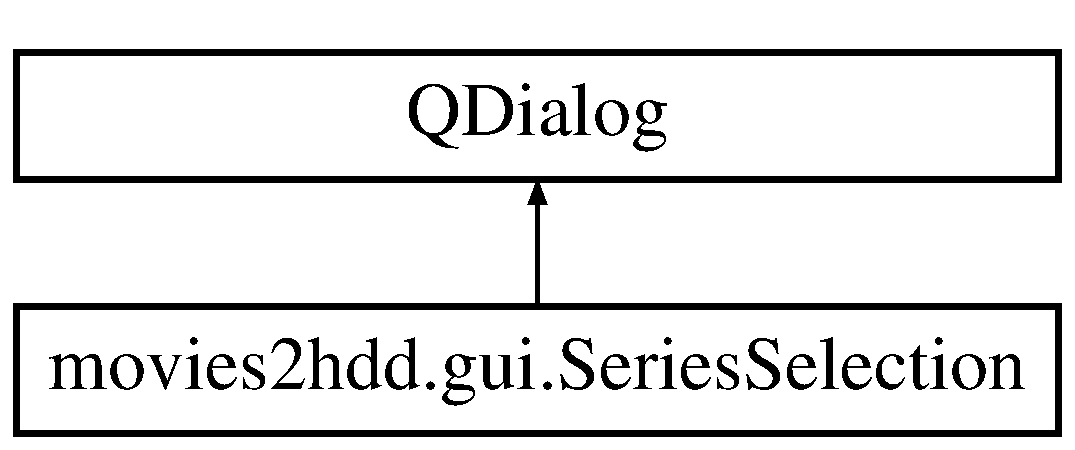
\includegraphics[height=2.000000cm]{classmovies2hdd_1_1gui_1_1_series_selection}
\end{center}
\end{figure}
\subsection*{Public Member Functions}
\begin{DoxyCompactItemize}
\item 
def \hyperlink{classmovies2hdd_1_1gui_1_1_series_selection_aa7aee53dd5df33e036a5bbffe99a903b}{\-\_\-\-\_\-init\-\_\-\-\_\-}
\item 
def \hyperlink{classmovies2hdd_1_1gui_1_1_series_selection_a59d9d53410754b1a797e2ec645c57591}{search\-For\-Series}
\item 
def \hyperlink{classmovies2hdd_1_1gui_1_1_series_selection_a97b0edb40452ba405e776132cae34997}{select}
\end{DoxyCompactItemize}
\subsection*{Public Attributes}
\begin{DoxyCompactItemize}
\item 
\hyperlink{classmovies2hdd_1_1gui_1_1_series_selection_a1d4759f70508c7fbcbf5ce849d6cee76}{layout}
\item 
\hyperlink{classmovies2hdd_1_1gui_1_1_series_selection_ae741cee9fe3b6d64c1e62413c063d7b1}{introduction}
\item 
\hyperlink{classmovies2hdd_1_1gui_1_1_series_selection_a514dd2b23706781594fe9d9886a28218}{form}
\item 
\hyperlink{classmovies2hdd_1_1gui_1_1_series_selection_a3ef4927decef147a124124515ab71114}{search\-Button}
\item 
\hyperlink{classmovies2hdd_1_1gui_1_1_series_selection_ac297f3ae5b7cbba9f01a3ebf7fa2fbb5}{table}
\item 
\hyperlink{classmovies2hdd_1_1gui_1_1_series_selection_ac43a1fd2985b12d7d42e5d3af24a5309}{button}
\end{DoxyCompactItemize}


\subsection{Detailed Description}


Definition at line 191 of file gui.\-py.



\subsection{Constructor \& Destructor Documentation}
\hypertarget{classmovies2hdd_1_1gui_1_1_series_selection_aa7aee53dd5df33e036a5bbffe99a903b}{\index{movies2hdd\-::gui\-::\-Series\-Selection@{movies2hdd\-::gui\-::\-Series\-Selection}!\-\_\-\-\_\-init\-\_\-\-\_\-@{\-\_\-\-\_\-init\-\_\-\-\_\-}}
\index{\-\_\-\-\_\-init\-\_\-\-\_\-@{\-\_\-\-\_\-init\-\_\-\-\_\-}!movies2hdd::gui::SeriesSelection@{movies2hdd\-::gui\-::\-Series\-Selection}}
\subsubsection[{\-\_\-\-\_\-init\-\_\-\-\_\-}]{\setlength{\rightskip}{0pt plus 5cm}def movies2hdd.\-gui.\-Series\-Selection.\-\_\-\-\_\-init\-\_\-\-\_\- (
\begin{DoxyParamCaption}
\item[{}]{self, }
\item[{}]{parent}
\end{DoxyParamCaption}
)}}\label{classmovies2hdd_1_1gui_1_1_series_selection_aa7aee53dd5df33e036a5bbffe99a903b}


Definition at line 192 of file gui.\-py.


\begin{DoxyCode}
192 
193         \textcolor{keyword}{def }\hyperlink{classmovies2hdd_1_1gui_1_1_series_selection_aa7aee53dd5df33e036a5bbffe99a903b}{\_\_init\_\_}(self, parent):
194             super(SeriesSelection, self).\hyperlink{classmovies2hdd_1_1gui_1_1_series_selection_aa7aee53dd5df33e036a5bbffe99a903b}{\_\_init\_\_}(parent)
195             self.setWindowTitle(\textcolor{stringliteral}{"Series Selection"})
196             self.\hyperlink{classmovies2hdd_1_1gui_1_1_series_selection_a1d4759f70508c7fbcbf5ce849d6cee76}{layout} = QVBoxLayout()
197             self.\hyperlink{classmovies2hdd_1_1gui_1_1_series_selection_ae741cee9fe3b6d64c1e62413c063d7b1}{introduction} = QLabel(\textcolor{stringliteral}{"Please enter the name of the series to search for and
       the language code."})
198             self.introduction.setWordWrap(\textcolor{keyword}{True})
199             self.layout.addWidget(self.\hyperlink{classmovies2hdd_1_1gui_1_1_series_selection_ae741cee9fe3b6d64c1e62413c063d7b1}{introduction})
200             self.\hyperlink{classmovies2hdd_1_1gui_1_1_series_selection_a514dd2b23706781594fe9d9886a28218}{form} = QFormLayout()
201             self.form.series = QLineEdit()
202             self.form.addRow(self.tr(\textcolor{stringliteral}{"&Series:"}), self.form.series)
203             self.form.lang = QLineEdit()
204             self.form.addRow(self.tr(\textcolor{stringliteral}{"&Language code:"}), self.form.lang)
205             self.layout.addLayout(self.\hyperlink{classmovies2hdd_1_1gui_1_1_series_selection_a514dd2b23706781594fe9d9886a28218}{form})
206             self.\hyperlink{classmovies2hdd_1_1gui_1_1_series_selection_a3ef4927decef147a124124515ab71114}{searchButton} = QPushButton(\textcolor{stringliteral}{"Se&arch"})
207             self.layout.addWidget(self.\hyperlink{classmovies2hdd_1_1gui_1_1_series_selection_a3ef4927decef147a124124515ab71114}{searchButton})
208             self.searchButton.clicked.connect(self.\hyperlink{classmovies2hdd_1_1gui_1_1_series_selection_a59d9d53410754b1a797e2ec645c57591}{searchForSeries})
209 
210             self.\hyperlink{classmovies2hdd_1_1gui_1_1_series_selection_ac297f3ae5b7cbba9f01a3ebf7fa2fbb5}{table} = QTableWidget()
211             self.table.setColumnCount(3)
212             self.table.setHorizontalHeaderLabels([\textcolor{stringliteral}{"ID"}, \textcolor{stringliteral}{"Series"}, \textcolor{stringliteral}{"Overview"}])
213             self.layout.addWidget(self.\hyperlink{classmovies2hdd_1_1gui_1_1_series_selection_ac297f3ae5b7cbba9f01a3ebf7fa2fbb5}{table})
214 
215             self.\hyperlink{classmovies2hdd_1_1gui_1_1_series_selection_ac43a1fd2985b12d7d42e5d3af24a5309}{button} = QPushButton(\textcolor{stringliteral}{"Se&lect"})
216             self.layout.addWidget(self.\hyperlink{classmovies2hdd_1_1gui_1_1_series_selection_ac43a1fd2985b12d7d42e5d3af24a5309}{button})
217             self.button.clicked.connect(self.\hyperlink{classmovies2hdd_1_1gui_1_1_series_selection_a97b0edb40452ba405e776132cae34997}{select})
218 
219             self.setLayout(self.\hyperlink{classmovies2hdd_1_1gui_1_1_series_selection_a1d4759f70508c7fbcbf5ce849d6cee76}{layout})

\end{DoxyCode}


\subsection{Member Function Documentation}
\hypertarget{classmovies2hdd_1_1gui_1_1_series_selection_a59d9d53410754b1a797e2ec645c57591}{\index{movies2hdd\-::gui\-::\-Series\-Selection@{movies2hdd\-::gui\-::\-Series\-Selection}!search\-For\-Series@{search\-For\-Series}}
\index{search\-For\-Series@{search\-For\-Series}!movies2hdd::gui::SeriesSelection@{movies2hdd\-::gui\-::\-Series\-Selection}}
\subsubsection[{search\-For\-Series}]{\setlength{\rightskip}{0pt plus 5cm}def movies2hdd.\-gui.\-Series\-Selection.\-search\-For\-Series (
\begin{DoxyParamCaption}
\item[{}]{self}
\end{DoxyParamCaption}
)}}\label{classmovies2hdd_1_1gui_1_1_series_selection_a59d9d53410754b1a797e2ec645c57591}


Definition at line 220 of file gui.\-py.


\begin{DoxyCode}
220 
221         \textcolor{keyword}{def }\hyperlink{classmovies2hdd_1_1gui_1_1_series_selection_a59d9d53410754b1a797e2ec645c57591}{searchForSeries}(self):
222             \textcolor{comment}{#progress = QProgressDialog("Searching for the series...", "Close", 0, 1, self)}
223             \textcolor{comment}{#progress.setWindowModality(Qt.WindowModal)}
224             \textcolor{comment}{#progress.setWindowTitle("Movies2HDD")}
225             \textcolor{comment}{#progress.setAutoClose(False)}
226             \textcolor{comment}{#progress.setCancelButton(None)}
227             \textcolor{comment}{#progress.setMinimumDuration(0)}
228             \textcolor{comment}{#progress.show()}
229             \textcolor{comment}{#progress.setValue(0)}
230             \textcolor{keywordflow}{try}:
231                 series = movies2hdd.getSeries(self.form.series.text())
232                 \textcolor{comment}{#progress.setMaximum(series.\_\_len\_\_())}
233                 self.table.clear()
234                 self.table.setRowCount(0)
235                 self.table.setHorizontalHeaderLabels([\textcolor{stringliteral}{"ID"}, \textcolor{stringliteral}{"Series"}, \textcolor{stringliteral}{"Overview"}])
236                 \textcolor{keywordflow}{for} x \textcolor{keywordflow}{in} series:
237                     \textcolor{comment}{#progress.setValue(progress.value() + 1)}
238                     flags = int(Qt.ItemIsEnabled) \textcolor{comment}{#+ int(Qt.ItemIsSelectable)}
239                     self.table.setRowCount(self.table.rowCount() + 1)
240                     sidItem = QTableWidgetItem(x[\textcolor{stringliteral}{'seriesid'}])
241                     sidItem.setFlags(flags)
242                     self.table.setItem(self.table.rowCount() - 1, 0, sidItem)
243                     SeriesNameItem = QTableWidgetItem(x[\textcolor{stringliteral}{'SeriesName'}])
244                     SeriesNameItem.setFlags(flags)
245                     self.table.setItem(self.table.rowCount() - 1, 1, SeriesNameItem)
246                     OverviewItem = QTableWidgetItem(x[\textcolor{stringliteral}{'Overview'}].replace(\textcolor{stringliteral}{"\(\backslash\)n"}, \textcolor{stringliteral}{"   "}))
247                     OverviewItem.setFlags(flags)
248                     self.table.setItem(self.table.rowCount() - 1, 2, OverviewItem)
249             \textcolor{keywordflow}{except} Exception \textcolor{keyword}{as} e:
250                 \textcolor{comment}{#sys.stderr.write("ERROR: " + str(e)+ "\(\backslash\)n")}
251                 msg.setText(\textcolor{stringliteral}{"An error occured.\(\backslash\)n\(\backslash\)nThe detailed error message is:\(\backslash\)n"}+str(e))
252                 msg.show()
253                 \textcolor{comment}{#progress.hide()}
254                 \textcolor{keywordflow}{raise}
255 

\end{DoxyCode}
\hypertarget{classmovies2hdd_1_1gui_1_1_series_selection_a97b0edb40452ba405e776132cae34997}{\index{movies2hdd\-::gui\-::\-Series\-Selection@{movies2hdd\-::gui\-::\-Series\-Selection}!select@{select}}
\index{select@{select}!movies2hdd::gui::SeriesSelection@{movies2hdd\-::gui\-::\-Series\-Selection}}
\subsubsection[{select}]{\setlength{\rightskip}{0pt plus 5cm}def movies2hdd.\-gui.\-Series\-Selection.\-select (
\begin{DoxyParamCaption}
\item[{}]{self}
\end{DoxyParamCaption}
)}}\label{classmovies2hdd_1_1gui_1_1_series_selection_a97b0edb40452ba405e776132cae34997}


Definition at line 256 of file gui.\-py.


\begin{DoxyCode}
256 
257         \textcolor{keyword}{def }\hyperlink{classmovies2hdd_1_1gui_1_1_series_selection_a97b0edb40452ba405e776132cae34997}{select}(self):
258             if(self.form.lang.text()!= \textcolor{stringliteral}{""}):
259                 \textcolor{keywordflow}{try}:
260                     item = self.table.item(self.table.currentRow(), 0)
261                     \textcolor{comment}{#The conversion str->int->str is not really needed. And it is nothing that the user can
       change. But it could prevent future issues.}
262                     sid = str(int(item.text()))
263                     self.parent().series\_selection.setText(sid)
264                     self.parent().setField(\textcolor{stringliteral}{"seriesid"}, sid)
265                     self.parent().setField(\textcolor{stringliteral}{"lang"}, self.form.lang.text())
266                     self.close()
267                 \textcolor{keywordflow}{except}:
268                     msg.setText(\textcolor{stringliteral}{"You need to select one series by clicking on it."})
269                     msg.show()
270             \textcolor{keywordflow}{else}:
271                 msg.setText(\textcolor{stringliteral}{"You need to enter your language code."})
272                 msg.show()
273 

\end{DoxyCode}


\subsection{Member Data Documentation}
\hypertarget{classmovies2hdd_1_1gui_1_1_series_selection_ac43a1fd2985b12d7d42e5d3af24a5309}{\index{movies2hdd\-::gui\-::\-Series\-Selection@{movies2hdd\-::gui\-::\-Series\-Selection}!button@{button}}
\index{button@{button}!movies2hdd::gui::SeriesSelection@{movies2hdd\-::gui\-::\-Series\-Selection}}
\subsubsection[{button}]{\setlength{\rightskip}{0pt plus 5cm}movies2hdd.\-gui.\-Series\-Selection.\-button}}\label{classmovies2hdd_1_1gui_1_1_series_selection_ac43a1fd2985b12d7d42e5d3af24a5309}


Definition at line 214 of file gui.\-py.

\hypertarget{classmovies2hdd_1_1gui_1_1_series_selection_a514dd2b23706781594fe9d9886a28218}{\index{movies2hdd\-::gui\-::\-Series\-Selection@{movies2hdd\-::gui\-::\-Series\-Selection}!form@{form}}
\index{form@{form}!movies2hdd::gui::SeriesSelection@{movies2hdd\-::gui\-::\-Series\-Selection}}
\subsubsection[{form}]{\setlength{\rightskip}{0pt plus 5cm}movies2hdd.\-gui.\-Series\-Selection.\-form}}\label{classmovies2hdd_1_1gui_1_1_series_selection_a514dd2b23706781594fe9d9886a28218}


Definition at line 199 of file gui.\-py.

\hypertarget{classmovies2hdd_1_1gui_1_1_series_selection_ae741cee9fe3b6d64c1e62413c063d7b1}{\index{movies2hdd\-::gui\-::\-Series\-Selection@{movies2hdd\-::gui\-::\-Series\-Selection}!introduction@{introduction}}
\index{introduction@{introduction}!movies2hdd::gui::SeriesSelection@{movies2hdd\-::gui\-::\-Series\-Selection}}
\subsubsection[{introduction}]{\setlength{\rightskip}{0pt plus 5cm}movies2hdd.\-gui.\-Series\-Selection.\-introduction}}\label{classmovies2hdd_1_1gui_1_1_series_selection_ae741cee9fe3b6d64c1e62413c063d7b1}


Definition at line 196 of file gui.\-py.

\hypertarget{classmovies2hdd_1_1gui_1_1_series_selection_a1d4759f70508c7fbcbf5ce849d6cee76}{\index{movies2hdd\-::gui\-::\-Series\-Selection@{movies2hdd\-::gui\-::\-Series\-Selection}!layout@{layout}}
\index{layout@{layout}!movies2hdd::gui::SeriesSelection@{movies2hdd\-::gui\-::\-Series\-Selection}}
\subsubsection[{layout}]{\setlength{\rightskip}{0pt plus 5cm}movies2hdd.\-gui.\-Series\-Selection.\-layout}}\label{classmovies2hdd_1_1gui_1_1_series_selection_a1d4759f70508c7fbcbf5ce849d6cee76}


Definition at line 195 of file gui.\-py.

\hypertarget{classmovies2hdd_1_1gui_1_1_series_selection_a3ef4927decef147a124124515ab71114}{\index{movies2hdd\-::gui\-::\-Series\-Selection@{movies2hdd\-::gui\-::\-Series\-Selection}!search\-Button@{search\-Button}}
\index{search\-Button@{search\-Button}!movies2hdd::gui::SeriesSelection@{movies2hdd\-::gui\-::\-Series\-Selection}}
\subsubsection[{search\-Button}]{\setlength{\rightskip}{0pt plus 5cm}movies2hdd.\-gui.\-Series\-Selection.\-search\-Button}}\label{classmovies2hdd_1_1gui_1_1_series_selection_a3ef4927decef147a124124515ab71114}


Definition at line 205 of file gui.\-py.

\hypertarget{classmovies2hdd_1_1gui_1_1_series_selection_ac297f3ae5b7cbba9f01a3ebf7fa2fbb5}{\index{movies2hdd\-::gui\-::\-Series\-Selection@{movies2hdd\-::gui\-::\-Series\-Selection}!table@{table}}
\index{table@{table}!movies2hdd::gui::SeriesSelection@{movies2hdd\-::gui\-::\-Series\-Selection}}
\subsubsection[{table}]{\setlength{\rightskip}{0pt plus 5cm}movies2hdd.\-gui.\-Series\-Selection.\-table}}\label{classmovies2hdd_1_1gui_1_1_series_selection_ac297f3ae5b7cbba9f01a3ebf7fa2fbb5}


Definition at line 209 of file gui.\-py.



The documentation for this class was generated from the following file\-:\begin{DoxyCompactItemize}
\item 
movies2hdd/\hyperlink{gui_8py}{gui.\-py}\end{DoxyCompactItemize}

\hypertarget{classmovies2hdd_1_1gui_1_1_step1}{\section{movies2hdd.\-gui.\-Step1 Class Reference}
\label{classmovies2hdd_1_1gui_1_1_step1}\index{movies2hdd.\-gui.\-Step1@{movies2hdd.\-gui.\-Step1}}
}
Inheritance diagram for movies2hdd.\-gui.\-Step1\-:\begin{figure}[H]
\begin{center}
\leavevmode
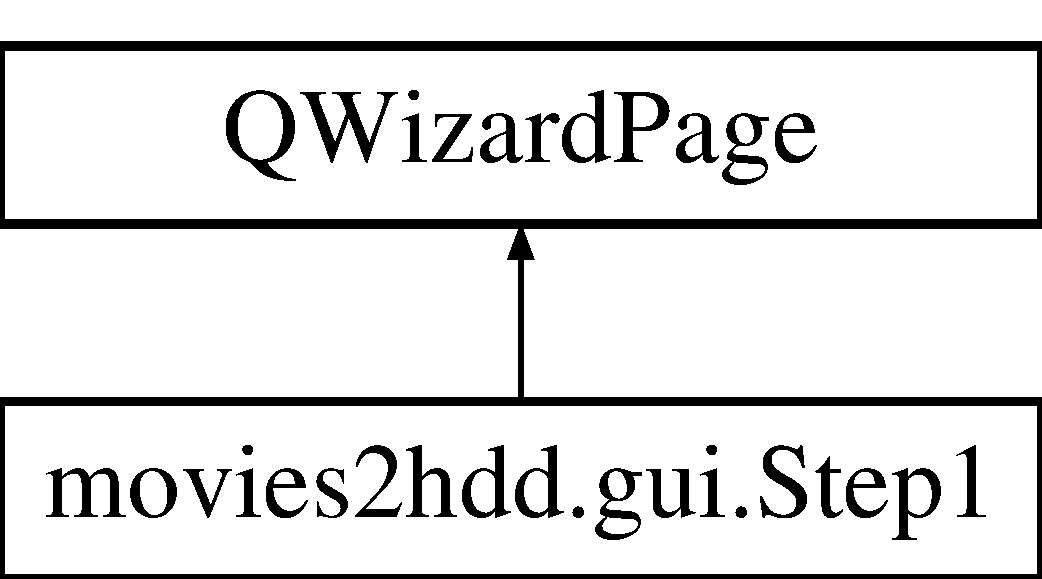
\includegraphics[height=2.000000cm]{classmovies2hdd_1_1gui_1_1_step1}
\end{center}
\end{figure}
\subsection*{Public Member Functions}
\begin{DoxyCompactItemize}
\item 
def \hyperlink{classmovies2hdd_1_1gui_1_1_step1_a7f77eb118cf3ec7debd009cdcedacb8f}{\-\_\-\-\_\-init\-\_\-\-\_\-}
\item 
def \hyperlink{classmovies2hdd_1_1gui_1_1_step1_a3268d2a740327b03b1af10c02ae6e10e}{func\-\_\-folder\-\_\-selection}
\item 
def \hyperlink{classmovies2hdd_1_1gui_1_1_step1_a93e5715186ec42ee18c1c5a0f75c54c4}{func\-\_\-series\-\_\-selection}
\item 
def \hyperlink{classmovies2hdd_1_1gui_1_1_step1_a4e623adf8d17a21563f58250e0fc4996}{validate\-Page}
\end{DoxyCompactItemize}
\subsection*{Public Attributes}
\begin{DoxyCompactItemize}
\item 
\hyperlink{classmovies2hdd_1_1gui_1_1_step1_ac872defae6a2ec8fa87724017327180f}{layout}
\item 
\hyperlink{classmovies2hdd_1_1gui_1_1_step1_a682a18695266e8fecbd3df9151f76e4a}{introduction}
\item 
\hyperlink{classmovies2hdd_1_1gui_1_1_step1_adef1bafe9ac90f458d6ef9597b3248b9}{form}
\item 
\hyperlink{classmovies2hdd_1_1gui_1_1_step1_a88c314f92883ddbe7c73ef89f7925929}{folder\-\_\-selection}
\item 
\hyperlink{classmovies2hdd_1_1gui_1_1_step1_a7de4eabf338df8f4e5ebad68f8235d78}{series\-\_\-selection}
\item 
\hyperlink{classmovies2hdd_1_1gui_1_1_step1_abd8a0c304da63971d4941db343634d11}{lang}
\end{DoxyCompactItemize}


\subsection{Detailed Description}


Definition at line 47 of file gui.\-py.



\subsection{Constructor \& Destructor Documentation}
\hypertarget{classmovies2hdd_1_1gui_1_1_step1_a7f77eb118cf3ec7debd009cdcedacb8f}{\index{movies2hdd\-::gui\-::\-Step1@{movies2hdd\-::gui\-::\-Step1}!\-\_\-\-\_\-init\-\_\-\-\_\-@{\-\_\-\-\_\-init\-\_\-\-\_\-}}
\index{\-\_\-\-\_\-init\-\_\-\-\_\-@{\-\_\-\-\_\-init\-\_\-\-\_\-}!movies2hdd::gui::Step1@{movies2hdd\-::gui\-::\-Step1}}
\subsubsection[{\-\_\-\-\_\-init\-\_\-\-\_\-}]{\setlength{\rightskip}{0pt plus 5cm}def movies2hdd.\-gui.\-Step1.\-\_\-\-\_\-init\-\_\-\-\_\- (
\begin{DoxyParamCaption}
\item[{}]{self, }
\item[{}]{parent = {\ttfamily None}}
\end{DoxyParamCaption}
)}}\label{classmovies2hdd_1_1gui_1_1_step1_a7f77eb118cf3ec7debd009cdcedacb8f}


Definition at line 48 of file gui.\-py.


\begin{DoxyCode}
48 
49     \textcolor{keyword}{def }\hyperlink{classmovies2hdd_1_1gui_1_1_step1_a7f77eb118cf3ec7debd009cdcedacb8f}{\_\_init\_\_}(self, parent=None):
50         super(Step1, self).\hyperlink{classmovies2hdd_1_1gui_1_1_step1_a7f77eb118cf3ec7debd009cdcedacb8f}{\_\_init\_\_}(parent)
51         self.setTitle(\textcolor{stringliteral}{"Select the folder and the series"})
52         self.\hyperlink{classmovies2hdd_1_1gui_1_1_step1_ac872defae6a2ec8fa87724017327180f}{layout} = QVBoxLayout()
53         self.\hyperlink{classmovies2hdd_1_1gui_1_1_step1_a682a18695266e8fecbd3df9151f76e4a}{introduction} = QLabel(\textcolor{stringliteral}{"First, you need to select the folder where the movies are
       or should be placed. The name of the series is needed, too."})
54         self.introduction.setWordWrap(\textcolor{keyword}{True})
55         self.layout.addWidget(self.\hyperlink{classmovies2hdd_1_1gui_1_1_step1_a682a18695266e8fecbd3df9151f76e4a}{introduction})
56         self.\hyperlink{classmovies2hdd_1_1gui_1_1_step1_adef1bafe9ac90f458d6ef9597b3248b9}{form} = QFormLayout()
57         self.\hyperlink{classmovies2hdd_1_1gui_1_1_step1_a88c314f92883ddbe7c73ef89f7925929}{folder\_selection} = QPushButton(\textcolor{stringliteral}{"Select"})
58         self.registerField(\textcolor{stringliteral}{"folder\_selection"}, self.\hyperlink{classmovies2hdd_1_1gui_1_1_step1_a88c314f92883ddbe7c73ef89f7925929}{folder\_selection})
59         self.folder\_selection.clicked.connect(self.\hyperlink{classmovies2hdd_1_1gui_1_1_step1_a3268d2a740327b03b1af10c02ae6e10e}{func\_folder\_selection})
60         self.form.addRow(self.tr(\textcolor{stringliteral}{"Select &folder:"}), self.\hyperlink{classmovies2hdd_1_1gui_1_1_step1_a88c314f92883ddbe7c73ef89f7925929}{folder\_selection})
61         self.\hyperlink{classmovies2hdd_1_1gui_1_1_step1_a7de4eabf338df8f4e5ebad68f8235d78}{series\_selection} = QPushButton(\textcolor{stringliteral}{"Select"})
62         self.registerField(\textcolor{stringliteral}{"seriesid"}, self.\hyperlink{classmovies2hdd_1_1gui_1_1_step1_a7de4eabf338df8f4e5ebad68f8235d78}{series\_selection})
63         self.series\_selection.clicked.connect(self.\hyperlink{classmovies2hdd_1_1gui_1_1_step1_a93e5715186ec42ee18c1c5a0f75c54c4}{func\_series\_selection})
64         self.form.addRow(self.tr(\textcolor{stringliteral}{"Select &series:"}), self.\hyperlink{classmovies2hdd_1_1gui_1_1_step1_a7de4eabf338df8f4e5ebad68f8235d78}{series\_selection})
65         self.layout.addLayout(self.\hyperlink{classmovies2hdd_1_1gui_1_1_step1_adef1bafe9ac90f458d6ef9597b3248b9}{form})
66         self.setLayout(self.\hyperlink{classmovies2hdd_1_1gui_1_1_step1_ac872defae6a2ec8fa87724017327180f}{layout})
67 
68         self.\hyperlink{classmovies2hdd_1_1gui_1_1_step1_abd8a0c304da63971d4941db343634d11}{lang} = QLineEdit()
69         self.registerField(\textcolor{stringliteral}{"lang"}, self.\hyperlink{classmovies2hdd_1_1gui_1_1_step1_abd8a0c304da63971d4941db343634d11}{lang})
70 

\end{DoxyCode}


\subsection{Member Function Documentation}
\hypertarget{classmovies2hdd_1_1gui_1_1_step1_a3268d2a740327b03b1af10c02ae6e10e}{\index{movies2hdd\-::gui\-::\-Step1@{movies2hdd\-::gui\-::\-Step1}!func\-\_\-folder\-\_\-selection@{func\-\_\-folder\-\_\-selection}}
\index{func\-\_\-folder\-\_\-selection@{func\-\_\-folder\-\_\-selection}!movies2hdd::gui::Step1@{movies2hdd\-::gui\-::\-Step1}}
\subsubsection[{func\-\_\-folder\-\_\-selection}]{\setlength{\rightskip}{0pt plus 5cm}def movies2hdd.\-gui.\-Step1.\-func\-\_\-folder\-\_\-selection (
\begin{DoxyParamCaption}
\item[{}]{self}
\end{DoxyParamCaption}
)}}\label{classmovies2hdd_1_1gui_1_1_step1_a3268d2a740327b03b1af10c02ae6e10e}


Definition at line 71 of file gui.\-py.


\begin{DoxyCode}
71 
72     \textcolor{keyword}{def }\hyperlink{classmovies2hdd_1_1gui_1_1_step1_a3268d2a740327b03b1af10c02ae6e10e}{func\_folder\_selection}(self):
73         folder = QFileDialog.getExistingDirectory()
74         self.folder\_selection.setText(folder)
75         self.setField(\textcolor{stringliteral}{"folder\_selection"}, folder)

\end{DoxyCode}
\hypertarget{classmovies2hdd_1_1gui_1_1_step1_a93e5715186ec42ee18c1c5a0f75c54c4}{\index{movies2hdd\-::gui\-::\-Step1@{movies2hdd\-::gui\-::\-Step1}!func\-\_\-series\-\_\-selection@{func\-\_\-series\-\_\-selection}}
\index{func\-\_\-series\-\_\-selection@{func\-\_\-series\-\_\-selection}!movies2hdd::gui::Step1@{movies2hdd\-::gui\-::\-Step1}}
\subsubsection[{func\-\_\-series\-\_\-selection}]{\setlength{\rightskip}{0pt plus 5cm}def movies2hdd.\-gui.\-Step1.\-func\-\_\-series\-\_\-selection (
\begin{DoxyParamCaption}
\item[{}]{self}
\end{DoxyParamCaption}
)}}\label{classmovies2hdd_1_1gui_1_1_step1_a93e5715186ec42ee18c1c5a0f75c54c4}


Definition at line 76 of file gui.\-py.


\begin{DoxyCode}
76 
77     \textcolor{keyword}{def }\hyperlink{classmovies2hdd_1_1gui_1_1_step1_a93e5715186ec42ee18c1c5a0f75c54c4}{func\_series\_selection}(self):
78         seriesselection = \hyperlink{classmovies2hdd_1_1gui_1_1_series_selection}{SeriesSelection}(self)
79         seriesselection.setWindowModality(Qt.WindowModal)
80         seriesselection.show()

\end{DoxyCode}
\hypertarget{classmovies2hdd_1_1gui_1_1_step1_a4e623adf8d17a21563f58250e0fc4996}{\index{movies2hdd\-::gui\-::\-Step1@{movies2hdd\-::gui\-::\-Step1}!validate\-Page@{validate\-Page}}
\index{validate\-Page@{validate\-Page}!movies2hdd::gui::Step1@{movies2hdd\-::gui\-::\-Step1}}
\subsubsection[{validate\-Page}]{\setlength{\rightskip}{0pt plus 5cm}def movies2hdd.\-gui.\-Step1.\-validate\-Page (
\begin{DoxyParamCaption}
\item[{}]{self}
\end{DoxyParamCaption}
)}}\label{classmovies2hdd_1_1gui_1_1_step1_a4e623adf8d17a21563f58250e0fc4996}


Definition at line 81 of file gui.\-py.


\begin{DoxyCode}
81 
82     \textcolor{keyword}{def }\hyperlink{classmovies2hdd_1_1gui_1_1_step1_a4e623adf8d17a21563f58250e0fc4996}{validatePage}(self):
83         \textcolor{keywordflow}{if} self.folder\_selection.text() != \textcolor{stringliteral}{"Select"} \textcolor{keywordflow}{and} self.\hyperlink{classmovies2hdd_1_1gui_1_1_step1_a7de4eabf338df8f4e5ebad68f8235d78}{series\_selection} != \textcolor{stringliteral}{"Select"} \textcolor{keywordflow}{
      and} self.folder\_selection.text() != \textcolor{stringliteral}{""}:
84             return(\textcolor{keyword}{True})
85         \textcolor{keywordflow}{else}:
86             msg.setText(\textcolor{stringliteral}{"You need to select a folder and a series first."})
87             msg.show()
88             return(\textcolor{keyword}{False})

\end{DoxyCode}


\subsection{Member Data Documentation}
\hypertarget{classmovies2hdd_1_1gui_1_1_step1_a88c314f92883ddbe7c73ef89f7925929}{\index{movies2hdd\-::gui\-::\-Step1@{movies2hdd\-::gui\-::\-Step1}!folder\-\_\-selection@{folder\-\_\-selection}}
\index{folder\-\_\-selection@{folder\-\_\-selection}!movies2hdd::gui::Step1@{movies2hdd\-::gui\-::\-Step1}}
\subsubsection[{folder\-\_\-selection}]{\setlength{\rightskip}{0pt plus 5cm}movies2hdd.\-gui.\-Step1.\-folder\-\_\-selection}}\label{classmovies2hdd_1_1gui_1_1_step1_a88c314f92883ddbe7c73ef89f7925929}


Definition at line 56 of file gui.\-py.

\hypertarget{classmovies2hdd_1_1gui_1_1_step1_adef1bafe9ac90f458d6ef9597b3248b9}{\index{movies2hdd\-::gui\-::\-Step1@{movies2hdd\-::gui\-::\-Step1}!form@{form}}
\index{form@{form}!movies2hdd::gui::Step1@{movies2hdd\-::gui\-::\-Step1}}
\subsubsection[{form}]{\setlength{\rightskip}{0pt plus 5cm}movies2hdd.\-gui.\-Step1.\-form}}\label{classmovies2hdd_1_1gui_1_1_step1_adef1bafe9ac90f458d6ef9597b3248b9}


Definition at line 55 of file gui.\-py.

\hypertarget{classmovies2hdd_1_1gui_1_1_step1_a682a18695266e8fecbd3df9151f76e4a}{\index{movies2hdd\-::gui\-::\-Step1@{movies2hdd\-::gui\-::\-Step1}!introduction@{introduction}}
\index{introduction@{introduction}!movies2hdd::gui::Step1@{movies2hdd\-::gui\-::\-Step1}}
\subsubsection[{introduction}]{\setlength{\rightskip}{0pt plus 5cm}movies2hdd.\-gui.\-Step1.\-introduction}}\label{classmovies2hdd_1_1gui_1_1_step1_a682a18695266e8fecbd3df9151f76e4a}


Definition at line 52 of file gui.\-py.

\hypertarget{classmovies2hdd_1_1gui_1_1_step1_abd8a0c304da63971d4941db343634d11}{\index{movies2hdd\-::gui\-::\-Step1@{movies2hdd\-::gui\-::\-Step1}!lang@{lang}}
\index{lang@{lang}!movies2hdd::gui::Step1@{movies2hdd\-::gui\-::\-Step1}}
\subsubsection[{lang}]{\setlength{\rightskip}{0pt plus 5cm}movies2hdd.\-gui.\-Step1.\-lang}}\label{classmovies2hdd_1_1gui_1_1_step1_abd8a0c304da63971d4941db343634d11}


Definition at line 67 of file gui.\-py.

\hypertarget{classmovies2hdd_1_1gui_1_1_step1_ac872defae6a2ec8fa87724017327180f}{\index{movies2hdd\-::gui\-::\-Step1@{movies2hdd\-::gui\-::\-Step1}!layout@{layout}}
\index{layout@{layout}!movies2hdd::gui::Step1@{movies2hdd\-::gui\-::\-Step1}}
\subsubsection[{layout}]{\setlength{\rightskip}{0pt plus 5cm}movies2hdd.\-gui.\-Step1.\-layout}}\label{classmovies2hdd_1_1gui_1_1_step1_ac872defae6a2ec8fa87724017327180f}


Definition at line 51 of file gui.\-py.

\hypertarget{classmovies2hdd_1_1gui_1_1_step1_a7de4eabf338df8f4e5ebad68f8235d78}{\index{movies2hdd\-::gui\-::\-Step1@{movies2hdd\-::gui\-::\-Step1}!series\-\_\-selection@{series\-\_\-selection}}
\index{series\-\_\-selection@{series\-\_\-selection}!movies2hdd::gui::Step1@{movies2hdd\-::gui\-::\-Step1}}
\subsubsection[{series\-\_\-selection}]{\setlength{\rightskip}{0pt plus 5cm}movies2hdd.\-gui.\-Step1.\-series\-\_\-selection}}\label{classmovies2hdd_1_1gui_1_1_step1_a7de4eabf338df8f4e5ebad68f8235d78}


Definition at line 60 of file gui.\-py.



The documentation for this class was generated from the following file\-:\begin{DoxyCompactItemize}
\item 
movies2hdd/\hyperlink{gui_8py}{gui.\-py}\end{DoxyCompactItemize}

\hypertarget{classmovies2hdd_1_1gui_1_1_step2}{\section{movies2hdd.\-gui.\-Step2 Class Reference}
\label{classmovies2hdd_1_1gui_1_1_step2}\index{movies2hdd.\-gui.\-Step2@{movies2hdd.\-gui.\-Step2}}
}
Inheritance diagram for movies2hdd.\-gui.\-Step2\-:\begin{figure}[H]
\begin{center}
\leavevmode
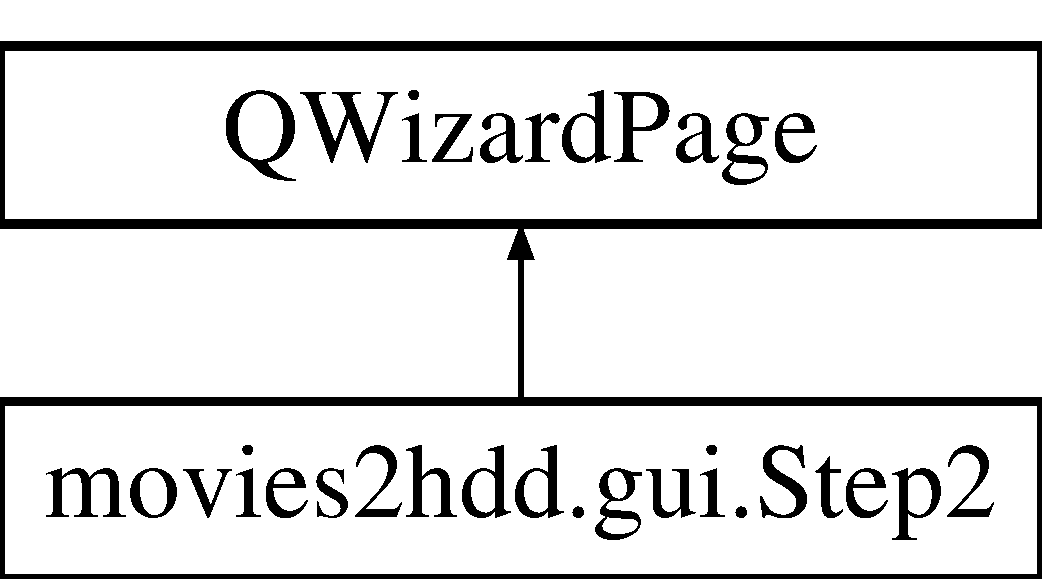
\includegraphics[height=2.000000cm]{classmovies2hdd_1_1gui_1_1_step2}
\end{center}
\end{figure}
\subsection*{Public Member Functions}
\begin{DoxyCompactItemize}
\item 
def \hyperlink{classmovies2hdd_1_1gui_1_1_step2_adbcd30dbde1136bd162a892ee16f6584}{\-\_\-\-\_\-init\-\_\-\-\_\-}
\item 
def \hyperlink{classmovies2hdd_1_1gui_1_1_step2_a9edb6b6d3a228791366c2003c7b17edf}{func\-\_\-check}
\item 
def \hyperlink{classmovies2hdd_1_1gui_1_1_step2_a5c46ff531c08753f9dca56f3e15717c0}{validate\-Page}
\item 
def \hyperlink{classmovies2hdd_1_1gui_1_1_step2_a9c39ae8418c352068f6248843eefe1f5}{next\-Id}
\end{DoxyCompactItemize}
\subsection*{Public Attributes}
\begin{DoxyCompactItemize}
\item 
\hyperlink{classmovies2hdd_1_1gui_1_1_step2_a0a18ea7d6f2a66251b60d74b8af0696b}{layout}
\item 
\hyperlink{classmovies2hdd_1_1gui_1_1_step2_af460b9a80cc6f30892480537debd47f9}{check}
\item 
\hyperlink{classmovies2hdd_1_1gui_1_1_step2_ac4656ee08d1176420516f83a856b0799}{group}
\item 
\hyperlink{classmovies2hdd_1_1gui_1_1_step2_a683a7687252c2018725e11630076d804}{host}
\item 
\hyperlink{classmovies2hdd_1_1gui_1_1_step2_a18455a364c4876707a596f250568abce}{user}
\item 
\hyperlink{classmovies2hdd_1_1gui_1_1_step2_a87c68120beaf76279360a47159d5c7aa}{warning}
\item 
\hyperlink{classmovies2hdd_1_1gui_1_1_step2_a3f46e0dc9e59cbc475fb08f1ab5c96e0}{password}
\end{DoxyCompactItemize}


\subsection{Detailed Description}


Definition at line 89 of file gui.\-py.



\subsection{Constructor \& Destructor Documentation}
\hypertarget{classmovies2hdd_1_1gui_1_1_step2_adbcd30dbde1136bd162a892ee16f6584}{\index{movies2hdd\-::gui\-::\-Step2@{movies2hdd\-::gui\-::\-Step2}!\-\_\-\-\_\-init\-\_\-\-\_\-@{\-\_\-\-\_\-init\-\_\-\-\_\-}}
\index{\-\_\-\-\_\-init\-\_\-\-\_\-@{\-\_\-\-\_\-init\-\_\-\-\_\-}!movies2hdd::gui::Step2@{movies2hdd\-::gui\-::\-Step2}}
\subsubsection[{\-\_\-\-\_\-init\-\_\-\-\_\-}]{\setlength{\rightskip}{0pt plus 5cm}def movies2hdd.\-gui.\-Step2.\-\_\-\-\_\-init\-\_\-\-\_\- (
\begin{DoxyParamCaption}
\item[{}]{self, }
\item[{}]{parent = {\ttfamily None}}
\end{DoxyParamCaption}
)}}\label{classmovies2hdd_1_1gui_1_1_step2_adbcd30dbde1136bd162a892ee16f6584}


Definition at line 90 of file gui.\-py.


\begin{DoxyCode}
90 
91     \textcolor{keyword}{def }\hyperlink{classmovies2hdd_1_1gui_1_1_step2_adbcd30dbde1136bd162a892ee16f6584}{\_\_init\_\_}(self, parent=None):
92         super(Step2, self).\hyperlink{classmovies2hdd_1_1gui_1_1_step2_adbcd30dbde1136bd162a892ee16f6584}{\_\_init\_\_}(parent)
93         self.setTitle(\textcolor{stringliteral}{"Connect to your Dreambox"})
94         self.\hyperlink{classmovies2hdd_1_1gui_1_1_step2_a0a18ea7d6f2a66251b60d74b8af0696b}{layout} = QVBoxLayout()
95         \textcolor{comment}{#self.introduction = QLabel("")}
96         \textcolor{comment}{#self.introduction.setWordWrap(True)}
97         \textcolor{comment}{#self.layout.addWidget(self.introduction)}
98         self.\hyperlink{classmovies2hdd_1_1gui_1_1_step2_af460b9a80cc6f30892480537debd47f9}{check} = QCheckBox(\textcolor{stringliteral}{"Do the movies need to be &downloaded?"})
99         self.check.stateChanged.connect(self.\hyperlink{classmovies2hdd_1_1gui_1_1_step2_a9edb6b6d3a228791366c2003c7b17edf}{func\_check})
100         self.layout.addWidget(self.\hyperlink{classmovies2hdd_1_1gui_1_1_step2_af460b9a80cc6f30892480537debd47f9}{check})
101 
102         self.\hyperlink{classmovies2hdd_1_1gui_1_1_step2_ac4656ee08d1176420516f83a856b0799}{group} = QGroupBox(\textcolor{stringliteral}{"Connection information"})
103         self.group.layout = QVBoxLayout()
104         self.group.form = QFormLayout()
105 
106         self.\hyperlink{classmovies2hdd_1_1gui_1_1_step2_a683a7687252c2018725e11630076d804}{host} = QLineEdit()
107         self.registerField(\textcolor{stringliteral}{"host"}, self.\hyperlink{classmovies2hdd_1_1gui_1_1_step2_a683a7687252c2018725e11630076d804}{host})
108         self.group.form.addRow(self.tr(\textcolor{stringliteral}{"&Host:"}), self.\hyperlink{classmovies2hdd_1_1gui_1_1_step2_a683a7687252c2018725e11630076d804}{host})
109         self.\hyperlink{classmovies2hdd_1_1gui_1_1_step2_a18455a364c4876707a596f250568abce}{user} = QLineEdit()
110         self.registerField(\textcolor{stringliteral}{"user"}, self.\hyperlink{classmovies2hdd_1_1gui_1_1_step2_a18455a364c4876707a596f250568abce}{user})
111         self.group.form.addRow(self.tr(\textcolor{stringliteral}{"&User:"}), self.\hyperlink{classmovies2hdd_1_1gui_1_1_step2_a18455a364c4876707a596f250568abce}{user})
112         self.\hyperlink{classmovies2hdd_1_1gui_1_1_step2_a87c68120beaf76279360a47159d5c7aa}{warning} = QLabel(\textcolor{stringliteral}{"<strong color='red'>Warning:</strong> Your password will be sent
       unencryptedly!\(\backslash\)nPlease do this only if you trust the network that you are currently connected to.\(\backslash\)nOtherwise
       please tunnel your connection for example via SSH or VPN."})
113         self.warning.setWordWrap(\textcolor{keyword}{True})
114         self.group.form.addRow(self.\hyperlink{classmovies2hdd_1_1gui_1_1_step2_a87c68120beaf76279360a47159d5c7aa}{warning})
115         self.\hyperlink{classmovies2hdd_1_1gui_1_1_step2_a3f46e0dc9e59cbc475fb08f1ab5c96e0}{password} = QLineEdit()
116         self.registerField(\textcolor{stringliteral}{"password"}, self.\hyperlink{classmovies2hdd_1_1gui_1_1_step2_a3f46e0dc9e59cbc475fb08f1ab5c96e0}{password})
117         self.password.setEchoMode(QLineEdit.EchoMode.Password)
118         self.group.form.addRow(self.tr(\textcolor{stringliteral}{"&Password:"}), self.\hyperlink{classmovies2hdd_1_1gui_1_1_step2_a3f46e0dc9e59cbc475fb08f1ab5c96e0}{password})
119 
120         self.group.layout.addLayout(self.group.form)
121         self.group.setLayout (self.group.layout)
122         self.layout.addWidget(self.\hyperlink{classmovies2hdd_1_1gui_1_1_step2_ac4656ee08d1176420516f83a856b0799}{group})
123         self.group.setEnabled(\textcolor{keyword}{False})
124 
125         self.setLayout(self.\hyperlink{classmovies2hdd_1_1gui_1_1_step2_a0a18ea7d6f2a66251b60d74b8af0696b}{layout})

\end{DoxyCode}


\subsection{Member Function Documentation}
\hypertarget{classmovies2hdd_1_1gui_1_1_step2_a9edb6b6d3a228791366c2003c7b17edf}{\index{movies2hdd\-::gui\-::\-Step2@{movies2hdd\-::gui\-::\-Step2}!func\-\_\-check@{func\-\_\-check}}
\index{func\-\_\-check@{func\-\_\-check}!movies2hdd::gui::Step2@{movies2hdd\-::gui\-::\-Step2}}
\subsubsection[{func\-\_\-check}]{\setlength{\rightskip}{0pt plus 5cm}def movies2hdd.\-gui.\-Step2.\-func\-\_\-check (
\begin{DoxyParamCaption}
\item[{}]{self}
\end{DoxyParamCaption}
)}}\label{classmovies2hdd_1_1gui_1_1_step2_a9edb6b6d3a228791366c2003c7b17edf}


Definition at line 126 of file gui.\-py.


\begin{DoxyCode}
126 
127     \textcolor{keyword}{def }\hyperlink{classmovies2hdd_1_1gui_1_1_step2_a9edb6b6d3a228791366c2003c7b17edf}{func\_check}(self):
128         self.group.setEnabled(self.check.isChecked())
129 

\end{DoxyCode}
\hypertarget{classmovies2hdd_1_1gui_1_1_step2_a9c39ae8418c352068f6248843eefe1f5}{\index{movies2hdd\-::gui\-::\-Step2@{movies2hdd\-::gui\-::\-Step2}!next\-Id@{next\-Id}}
\index{next\-Id@{next\-Id}!movies2hdd::gui::Step2@{movies2hdd\-::gui\-::\-Step2}}
\subsubsection[{next\-Id}]{\setlength{\rightskip}{0pt plus 5cm}def movies2hdd.\-gui.\-Step2.\-next\-Id (
\begin{DoxyParamCaption}
\item[{}]{self}
\end{DoxyParamCaption}
)}}\label{classmovies2hdd_1_1gui_1_1_step2_a9c39ae8418c352068f6248843eefe1f5}


Definition at line 144 of file gui.\-py.


\begin{DoxyCode}
144 
145     \textcolor{keyword}{def }\hyperlink{classmovies2hdd_1_1gui_1_1_step2_a9c39ae8418c352068f6248843eefe1f5}{nextId}(self):
146         \textcolor{keywordflow}{if} self.check.isChecked() == \textcolor{keyword}{False}:
147             return(3)
148         \textcolor{keywordflow}{else}:
149             return(2)

\end{DoxyCode}
\hypertarget{classmovies2hdd_1_1gui_1_1_step2_a5c46ff531c08753f9dca56f3e15717c0}{\index{movies2hdd\-::gui\-::\-Step2@{movies2hdd\-::gui\-::\-Step2}!validate\-Page@{validate\-Page}}
\index{validate\-Page@{validate\-Page}!movies2hdd::gui::Step2@{movies2hdd\-::gui\-::\-Step2}}
\subsubsection[{validate\-Page}]{\setlength{\rightskip}{0pt plus 5cm}def movies2hdd.\-gui.\-Step2.\-validate\-Page (
\begin{DoxyParamCaption}
\item[{}]{self}
\end{DoxyParamCaption}
)}}\label{classmovies2hdd_1_1gui_1_1_step2_a5c46ff531c08753f9dca56f3e15717c0}


Definition at line 130 of file gui.\-py.


\begin{DoxyCode}
130 
131     \textcolor{keyword}{def }\hyperlink{classmovies2hdd_1_1gui_1_1_step2_a5c46ff531c08753f9dca56f3e15717c0}{validatePage}(self):
132         \textcolor{keywordflow}{if} self.check.isChecked() == \textcolor{keyword}{False}:
133             return(\textcolor{keyword}{True})
134         \textcolor{keywordflow}{else}:
135             \textcolor{keywordflow}{try}:
136                 movies2hdd.connect(self.host.text(), self.user.text(), self.password.text())
137                 return(\textcolor{keyword}{True})
138             \textcolor{keywordflow}{except} Exception \textcolor{keyword}{as} e:
139                 \textcolor{comment}{#sys.stderr.write("ERROR: " + str(e) + "\(\backslash\)n")}
140                 msg.setText(\textcolor{stringliteral}{"Could not connect.\(\backslash\)nPlease check your input and your connection.\(\backslash\)n\(\backslash\)nThe
       detailed error message is:\(\backslash\)n"}+str(e))
141                 msg.show()
142                 \textcolor{keywordflow}{raise}
143                 return(\textcolor{keyword}{False})

\end{DoxyCode}


\subsection{Member Data Documentation}
\hypertarget{classmovies2hdd_1_1gui_1_1_step2_af460b9a80cc6f30892480537debd47f9}{\index{movies2hdd\-::gui\-::\-Step2@{movies2hdd\-::gui\-::\-Step2}!check@{check}}
\index{check@{check}!movies2hdd::gui::Step2@{movies2hdd\-::gui\-::\-Step2}}
\subsubsection[{check}]{\setlength{\rightskip}{0pt plus 5cm}movies2hdd.\-gui.\-Step2.\-check}}\label{classmovies2hdd_1_1gui_1_1_step2_af460b9a80cc6f30892480537debd47f9}


Definition at line 97 of file gui.\-py.

\hypertarget{classmovies2hdd_1_1gui_1_1_step2_ac4656ee08d1176420516f83a856b0799}{\index{movies2hdd\-::gui\-::\-Step2@{movies2hdd\-::gui\-::\-Step2}!group@{group}}
\index{group@{group}!movies2hdd::gui::Step2@{movies2hdd\-::gui\-::\-Step2}}
\subsubsection[{group}]{\setlength{\rightskip}{0pt plus 5cm}movies2hdd.\-gui.\-Step2.\-group}}\label{classmovies2hdd_1_1gui_1_1_step2_ac4656ee08d1176420516f83a856b0799}


Definition at line 101 of file gui.\-py.

\hypertarget{classmovies2hdd_1_1gui_1_1_step2_a683a7687252c2018725e11630076d804}{\index{movies2hdd\-::gui\-::\-Step2@{movies2hdd\-::gui\-::\-Step2}!host@{host}}
\index{host@{host}!movies2hdd::gui::Step2@{movies2hdd\-::gui\-::\-Step2}}
\subsubsection[{host}]{\setlength{\rightskip}{0pt plus 5cm}movies2hdd.\-gui.\-Step2.\-host}}\label{classmovies2hdd_1_1gui_1_1_step2_a683a7687252c2018725e11630076d804}


Definition at line 105 of file gui.\-py.

\hypertarget{classmovies2hdd_1_1gui_1_1_step2_a0a18ea7d6f2a66251b60d74b8af0696b}{\index{movies2hdd\-::gui\-::\-Step2@{movies2hdd\-::gui\-::\-Step2}!layout@{layout}}
\index{layout@{layout}!movies2hdd::gui::Step2@{movies2hdd\-::gui\-::\-Step2}}
\subsubsection[{layout}]{\setlength{\rightskip}{0pt plus 5cm}movies2hdd.\-gui.\-Step2.\-layout}}\label{classmovies2hdd_1_1gui_1_1_step2_a0a18ea7d6f2a66251b60d74b8af0696b}


Definition at line 93 of file gui.\-py.

\hypertarget{classmovies2hdd_1_1gui_1_1_step2_a3f46e0dc9e59cbc475fb08f1ab5c96e0}{\index{movies2hdd\-::gui\-::\-Step2@{movies2hdd\-::gui\-::\-Step2}!password@{password}}
\index{password@{password}!movies2hdd::gui::Step2@{movies2hdd\-::gui\-::\-Step2}}
\subsubsection[{password}]{\setlength{\rightskip}{0pt plus 5cm}movies2hdd.\-gui.\-Step2.\-password}}\label{classmovies2hdd_1_1gui_1_1_step2_a3f46e0dc9e59cbc475fb08f1ab5c96e0}


Definition at line 114 of file gui.\-py.

\hypertarget{classmovies2hdd_1_1gui_1_1_step2_a18455a364c4876707a596f250568abce}{\index{movies2hdd\-::gui\-::\-Step2@{movies2hdd\-::gui\-::\-Step2}!user@{user}}
\index{user@{user}!movies2hdd::gui::Step2@{movies2hdd\-::gui\-::\-Step2}}
\subsubsection[{user}]{\setlength{\rightskip}{0pt plus 5cm}movies2hdd.\-gui.\-Step2.\-user}}\label{classmovies2hdd_1_1gui_1_1_step2_a18455a364c4876707a596f250568abce}


Definition at line 108 of file gui.\-py.

\hypertarget{classmovies2hdd_1_1gui_1_1_step2_a87c68120beaf76279360a47159d5c7aa}{\index{movies2hdd\-::gui\-::\-Step2@{movies2hdd\-::gui\-::\-Step2}!warning@{warning}}
\index{warning@{warning}!movies2hdd::gui::Step2@{movies2hdd\-::gui\-::\-Step2}}
\subsubsection[{warning}]{\setlength{\rightskip}{0pt plus 5cm}movies2hdd.\-gui.\-Step2.\-warning}}\label{classmovies2hdd_1_1gui_1_1_step2_a87c68120beaf76279360a47159d5c7aa}


Definition at line 111 of file gui.\-py.



The documentation for this class was generated from the following file\-:\begin{DoxyCompactItemize}
\item 
movies2hdd/\hyperlink{gui_8py}{gui.\-py}\end{DoxyCompactItemize}

\hypertarget{classmovies2hdd_1_1gui_1_1_step3}{\section{movies2hdd.\-gui.\-Step3 Class Reference}
\label{classmovies2hdd_1_1gui_1_1_step3}\index{movies2hdd.\-gui.\-Step3@{movies2hdd.\-gui.\-Step3}}
}
Inheritance diagram for movies2hdd.\-gui.\-Step3\-:\begin{figure}[H]
\begin{center}
\leavevmode
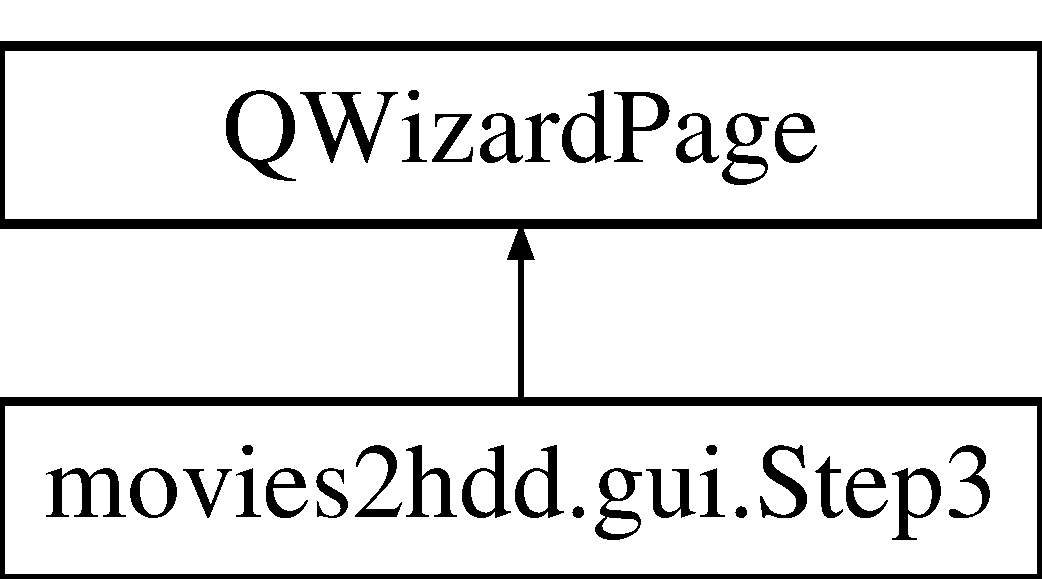
\includegraphics[height=2.000000cm]{classmovies2hdd_1_1gui_1_1_step3}
\end{center}
\end{figure}
\subsection*{Public Member Functions}
\begin{DoxyCompactItemize}
\item 
def \hyperlink{classmovies2hdd_1_1gui_1_1_step3_adced9712cc906ff656705527c0b5da48}{\-\_\-\-\_\-init\-\_\-\-\_\-}
\item 
def \hyperlink{classmovies2hdd_1_1gui_1_1_step3_ae1ba8bc0179241cd53633c532f28dc25}{func\-\_\-search}
\item 
def \hyperlink{classmovies2hdd_1_1gui_1_1_step3_abd850ebfb1a7b7bb76f70ffd178f9413}{validate\-Page}
\end{DoxyCompactItemize}
\subsection*{Public Attributes}
\begin{DoxyCompactItemize}
\item 
\hyperlink{classmovies2hdd_1_1gui_1_1_step3_a219925352b4ccaef913b4530039cefd3}{layout}
\item 
\hyperlink{classmovies2hdd_1_1gui_1_1_step3_acac006717bba2aa2f5834fecf3db359f}{introduction}
\item 
\hyperlink{classmovies2hdd_1_1gui_1_1_step3_affbacc9b3831417408811bd57aa7af76}{form}
\item 
\hyperlink{classmovies2hdd_1_1gui_1_1_step3_a7d8d7669f3636fb078fa022ebc1906bd}{line\-Edit}
\item 
\hyperlink{classmovies2hdd_1_1gui_1_1_step3_a3943ef1d0f93ffd6405996b301ec47d3}{push\-Button}
\item 
\hyperlink{classmovies2hdd_1_1gui_1_1_step3_ab2215782905268ba4287fa1872f1618e}{list}
\end{DoxyCompactItemize}


\subsection{Detailed Description}


Definition at line 150 of file gui.\-py.



\subsection{Constructor \& Destructor Documentation}
\hypertarget{classmovies2hdd_1_1gui_1_1_step3_adced9712cc906ff656705527c0b5da48}{\index{movies2hdd\-::gui\-::\-Step3@{movies2hdd\-::gui\-::\-Step3}!\-\_\-\-\_\-init\-\_\-\-\_\-@{\-\_\-\-\_\-init\-\_\-\-\_\-}}
\index{\-\_\-\-\_\-init\-\_\-\-\_\-@{\-\_\-\-\_\-init\-\_\-\-\_\-}!movies2hdd::gui::Step3@{movies2hdd\-::gui\-::\-Step3}}
\subsubsection[{\-\_\-\-\_\-init\-\_\-\-\_\-}]{\setlength{\rightskip}{0pt plus 5cm}def movies2hdd.\-gui.\-Step3.\-\_\-\-\_\-init\-\_\-\-\_\- (
\begin{DoxyParamCaption}
\item[{}]{self, }
\item[{}]{parent = {\ttfamily None}}
\end{DoxyParamCaption}
)}}\label{classmovies2hdd_1_1gui_1_1_step3_adced9712cc906ff656705527c0b5da48}


Definition at line 151 of file gui.\-py.


\begin{DoxyCode}
151 
152     \textcolor{keyword}{def }\hyperlink{classmovies2hdd_1_1gui_1_1_step3_adced9712cc906ff656705527c0b5da48}{\_\_init\_\_}(self, parent=None):
153         super(Step3, self).\hyperlink{classmovies2hdd_1_1gui_1_1_step3_adced9712cc906ff656705527c0b5da48}{\_\_init\_\_}(parent)
154         self.setTitle(\textcolor{stringliteral}{"Search for and select movies"})
155         self.\hyperlink{classmovies2hdd_1_1gui_1_1_step3_a219925352b4ccaef913b4530039cefd3}{layout} = QVBoxLayout()
156         self.\hyperlink{classmovies2hdd_1_1gui_1_1_step3_acac006717bba2aa2f5834fecf3db359f}{introduction} = QLabel(\textcolor{stringliteral}{"Please enter a string to search for:"})
157         self.introduction.setWordWrap(\textcolor{keyword}{True})
158         self.layout.addWidget(self.\hyperlink{classmovies2hdd_1_1gui_1_1_step3_acac006717bba2aa2f5834fecf3db359f}{introduction})
159         self.\hyperlink{classmovies2hdd_1_1gui_1_1_step3_affbacc9b3831417408811bd57aa7af76}{form} = QFormLayout()
160         self.\hyperlink{classmovies2hdd_1_1gui_1_1_step3_a7d8d7669f3636fb078fa022ebc1906bd}{lineEdit} = QLineEdit()
161         self.form.addRow(self.tr(\textcolor{stringliteral}{"&Search string:"}), self.\hyperlink{classmovies2hdd_1_1gui_1_1_step3_a7d8d7669f3636fb078fa022ebc1906bd}{lineEdit})
162         self.layout.addLayout(self.\hyperlink{classmovies2hdd_1_1gui_1_1_step3_affbacc9b3831417408811bd57aa7af76}{form})
163         self.\hyperlink{classmovies2hdd_1_1gui_1_1_step3_a3943ef1d0f93ffd6405996b301ec47d3}{pushButton} = QPushButton(\textcolor{stringliteral}{"S&earch"})
164         self.pushButton.clicked.connect(self.\hyperlink{classmovies2hdd_1_1gui_1_1_step3_ae1ba8bc0179241cd53633c532f28dc25}{func\_search})
165         self.layout.addWidget(self.\hyperlink{classmovies2hdd_1_1gui_1_1_step3_a3943ef1d0f93ffd6405996b301ec47d3}{pushButton})
166         self.\hyperlink{classmovies2hdd_1_1gui_1_1_step3_ab2215782905268ba4287fa1872f1618e}{list} = QListWidget()
167         self.layout.addWidget(self.\hyperlink{classmovies2hdd_1_1gui_1_1_step3_ab2215782905268ba4287fa1872f1618e}{list})
168         self.setLayout(self.\hyperlink{classmovies2hdd_1_1gui_1_1_step3_a219925352b4ccaef913b4530039cefd3}{layout})

\end{DoxyCode}


\subsection{Member Function Documentation}
\hypertarget{classmovies2hdd_1_1gui_1_1_step3_ae1ba8bc0179241cd53633c532f28dc25}{\index{movies2hdd\-::gui\-::\-Step3@{movies2hdd\-::gui\-::\-Step3}!func\-\_\-search@{func\-\_\-search}}
\index{func\-\_\-search@{func\-\_\-search}!movies2hdd::gui::Step3@{movies2hdd\-::gui\-::\-Step3}}
\subsubsection[{func\-\_\-search}]{\setlength{\rightskip}{0pt plus 5cm}def movies2hdd.\-gui.\-Step3.\-func\-\_\-search (
\begin{DoxyParamCaption}
\item[{}]{self}
\end{DoxyParamCaption}
)}}\label{classmovies2hdd_1_1gui_1_1_step3_ae1ba8bc0179241cd53633c532f28dc25}


Definition at line 169 of file gui.\-py.


\begin{DoxyCode}
169 
170     \textcolor{keyword}{def }\hyperlink{classmovies2hdd_1_1gui_1_1_step3_ae1ba8bc0179241cd53633c532f28dc25}{func\_search}(self):
171         self.list.clear()
172         movies = []
173         \textcolor{keywordflow}{try}:
174             movies = movies2hdd.getAviableMovies(self.lineEdit.text())
175         \textcolor{keywordflow}{except}:
176             \textcolor{keywordflow}{try}:
177                 movies2hdd.connect(self.field(\textcolor{stringliteral}{"host"}), self.field(\textcolor{stringliteral}{"user"}), self.field(\textcolor{stringliteral}{"password"}))
178                 movies = movies2hdd.getAviableMovies(str(\textcolor{stringliteral}{""}+self.lineEdit.text()))
179             \textcolor{keywordflow}{except} Exception \textcolor{keyword}{as} e:
180                 \textcolor{comment}{#sys.stderr.write("ERROR: " + str(e)+ "\(\backslash\)n")}
181                 msg.setText(\textcolor{stringliteral}{"Something went wrong.\(\backslash\)n\(\backslash\)nThe detailed error message is:\(\backslash\)n"}+str(e))
182                 msg.show()
183                 \textcolor{keywordflow}{raise}
184         \textcolor{keywordflow}{finally}:
185             \textcolor{keywordflow}{for} x \textcolor{keywordflow}{in} movies:
186                 self.list.addItem(QListWidgetItem(x))
187             

\end{DoxyCode}
\hypertarget{classmovies2hdd_1_1gui_1_1_step3_abd850ebfb1a7b7bb76f70ffd178f9413}{\index{movies2hdd\-::gui\-::\-Step3@{movies2hdd\-::gui\-::\-Step3}!validate\-Page@{validate\-Page}}
\index{validate\-Page@{validate\-Page}!movies2hdd::gui::Step3@{movies2hdd\-::gui\-::\-Step3}}
\subsubsection[{validate\-Page}]{\setlength{\rightskip}{0pt plus 5cm}def movies2hdd.\-gui.\-Step3.\-validate\-Page (
\begin{DoxyParamCaption}
\item[{}]{self}
\end{DoxyParamCaption}
)}}\label{classmovies2hdd_1_1gui_1_1_step3_abd850ebfb1a7b7bb76f70ffd178f9413}


Definition at line 188 of file gui.\-py.


\begin{DoxyCode}
188 
189     \textcolor{keyword}{def }\hyperlink{classmovies2hdd_1_1gui_1_1_step3_abd850ebfb1a7b7bb76f70ffd178f9413}{validatePage}(self):
190         return(\textcolor{keyword}{False})

\end{DoxyCode}


\subsection{Member Data Documentation}
\hypertarget{classmovies2hdd_1_1gui_1_1_step3_affbacc9b3831417408811bd57aa7af76}{\index{movies2hdd\-::gui\-::\-Step3@{movies2hdd\-::gui\-::\-Step3}!form@{form}}
\index{form@{form}!movies2hdd::gui::Step3@{movies2hdd\-::gui\-::\-Step3}}
\subsubsection[{form}]{\setlength{\rightskip}{0pt plus 5cm}movies2hdd.\-gui.\-Step3.\-form}}\label{classmovies2hdd_1_1gui_1_1_step3_affbacc9b3831417408811bd57aa7af76}


Definition at line 158 of file gui.\-py.

\hypertarget{classmovies2hdd_1_1gui_1_1_step3_acac006717bba2aa2f5834fecf3db359f}{\index{movies2hdd\-::gui\-::\-Step3@{movies2hdd\-::gui\-::\-Step3}!introduction@{introduction}}
\index{introduction@{introduction}!movies2hdd::gui::Step3@{movies2hdd\-::gui\-::\-Step3}}
\subsubsection[{introduction}]{\setlength{\rightskip}{0pt plus 5cm}movies2hdd.\-gui.\-Step3.\-introduction}}\label{classmovies2hdd_1_1gui_1_1_step3_acac006717bba2aa2f5834fecf3db359f}


Definition at line 155 of file gui.\-py.

\hypertarget{classmovies2hdd_1_1gui_1_1_step3_a219925352b4ccaef913b4530039cefd3}{\index{movies2hdd\-::gui\-::\-Step3@{movies2hdd\-::gui\-::\-Step3}!layout@{layout}}
\index{layout@{layout}!movies2hdd::gui::Step3@{movies2hdd\-::gui\-::\-Step3}}
\subsubsection[{layout}]{\setlength{\rightskip}{0pt plus 5cm}movies2hdd.\-gui.\-Step3.\-layout}}\label{classmovies2hdd_1_1gui_1_1_step3_a219925352b4ccaef913b4530039cefd3}


Definition at line 154 of file gui.\-py.

\hypertarget{classmovies2hdd_1_1gui_1_1_step3_a7d8d7669f3636fb078fa022ebc1906bd}{\index{movies2hdd\-::gui\-::\-Step3@{movies2hdd\-::gui\-::\-Step3}!line\-Edit@{line\-Edit}}
\index{line\-Edit@{line\-Edit}!movies2hdd::gui::Step3@{movies2hdd\-::gui\-::\-Step3}}
\subsubsection[{line\-Edit}]{\setlength{\rightskip}{0pt plus 5cm}movies2hdd.\-gui.\-Step3.\-line\-Edit}}\label{classmovies2hdd_1_1gui_1_1_step3_a7d8d7669f3636fb078fa022ebc1906bd}


Definition at line 159 of file gui.\-py.

\hypertarget{classmovies2hdd_1_1gui_1_1_step3_ab2215782905268ba4287fa1872f1618e}{\index{movies2hdd\-::gui\-::\-Step3@{movies2hdd\-::gui\-::\-Step3}!list@{list}}
\index{list@{list}!movies2hdd::gui::Step3@{movies2hdd\-::gui\-::\-Step3}}
\subsubsection[{list}]{\setlength{\rightskip}{0pt plus 5cm}movies2hdd.\-gui.\-Step3.\-list}}\label{classmovies2hdd_1_1gui_1_1_step3_ab2215782905268ba4287fa1872f1618e}


Definition at line 165 of file gui.\-py.

\hypertarget{classmovies2hdd_1_1gui_1_1_step3_a3943ef1d0f93ffd6405996b301ec47d3}{\index{movies2hdd\-::gui\-::\-Step3@{movies2hdd\-::gui\-::\-Step3}!push\-Button@{push\-Button}}
\index{push\-Button@{push\-Button}!movies2hdd::gui::Step3@{movies2hdd\-::gui\-::\-Step3}}
\subsubsection[{push\-Button}]{\setlength{\rightskip}{0pt plus 5cm}movies2hdd.\-gui.\-Step3.\-push\-Button}}\label{classmovies2hdd_1_1gui_1_1_step3_a3943ef1d0f93ffd6405996b301ec47d3}


Definition at line 162 of file gui.\-py.



The documentation for this class was generated from the following file\-:\begin{DoxyCompactItemize}
\item 
movies2hdd/\hyperlink{gui_8py}{gui.\-py}\end{DoxyCompactItemize}

\chapter{File Documentation}
\hypertarget{____init_____8py}{\section{movies2hdd/\-\_\-\-\_\-init\-\_\-\-\_\-.py File Reference}
\label{____init_____8py}\index{movies2hdd/\-\_\-\-\_\-init\-\_\-\-\_\-.\-py@{movies2hdd/\-\_\-\-\_\-init\-\_\-\-\_\-.\-py}}
}
\subsection*{Classes}
\begin{DoxyCompactItemize}
\item 
class \hyperlink{classmovies2hdd_1_1_movies2_h_d_d}{movies2hdd.\-Movies2\-H\-D\-D}
\end{DoxyCompactItemize}
\subsection*{Namespaces}
\begin{DoxyCompactItemize}
\item 
\hyperlink{namespacemovies2hdd}{movies2hdd}
\end{DoxyCompactItemize}
\subsection*{Constant Groups}
\begin{DoxyCompactItemize}
\item 
\hyperlink{namespacemovies2hdd}{movies2hdd}
\end{DoxyCompactItemize}

\hypertarget{convert_8py}{\section{movies2hdd/convert.py File Reference}
\label{convert_8py}\index{movies2hdd/convert.\-py@{movies2hdd/convert.\-py}}
}
\subsection*{Namespaces}
\begin{DoxyCompactItemize}
\item 
\hyperlink{namespacemovies2hdd_1_1convert}{movies2hdd.\-convert}
\end{DoxyCompactItemize}
\subsection*{Constant Groups}
\begin{DoxyCompactItemize}
\item 
\hyperlink{namespacemovies2hdd_1_1convert}{movies2hdd.\-convert}
\end{DoxyCompactItemize}
\subsection*{Variables}
\begin{DoxyCompactItemize}
\item 
list \hyperlink{namespacemovies2hdd_1_1convert_aa56ab068434359bf27101c2903a2a076}{movies2hdd.\-convert.\-movie} = sys.\-argv\mbox{[}1\mbox{]}
\end{DoxyCompactItemize}

\hypertarget{gui_8py}{\section{movies2hdd/gui.py File Reference}
\label{gui_8py}\index{movies2hdd/gui.\-py@{movies2hdd/gui.\-py}}
}
\subsection*{Classes}
\begin{DoxyCompactItemize}
\item 
class \hyperlink{classmovies2hdd_1_1gui_1_1_step1}{movies2hdd.\-gui.\-Step1}
\item 
class \hyperlink{classmovies2hdd_1_1gui_1_1_step2}{movies2hdd.\-gui.\-Step2}
\item 
class \hyperlink{classmovies2hdd_1_1gui_1_1_step3}{movies2hdd.\-gui.\-Step3}
\item 
class \hyperlink{classmovies2hdd_1_1gui_1_1_series_selection}{movies2hdd.\-gui.\-Series\-Selection}
\end{DoxyCompactItemize}
\subsection*{Namespaces}
\begin{DoxyCompactItemize}
\item 
\hyperlink{namespacemovies2hdd_1_1gui}{movies2hdd.\-gui}
\end{DoxyCompactItemize}
\subsection*{Constant Groups}
\begin{DoxyCompactItemize}
\item 
\hyperlink{namespacemovies2hdd_1_1gui}{movies2hdd.\-gui}
\end{DoxyCompactItemize}
\subsection*{Variables}
\begin{DoxyCompactItemize}
\item 
tuple \hyperlink{namespacemovies2hdd_1_1gui_a5113ba41da39d51855bd15d8cf47d7be}{movies2hdd.\-gui.\-app} = Q\-Application(sys.\-argv)
\item 
tuple \hyperlink{namespacemovies2hdd_1_1gui_a04dfe049e2e7207b12600d74a0b13749}{movies2hdd.\-gui.\-msg} = Q\-Message\-Box()
\item 
tuple \hyperlink{namespacemovies2hdd_1_1gui_a186ac0ab862ac5332f6dfc3e927126f0}{movies2hdd.\-gui.\-movies2hdd} = Movies2\-H\-D\-D()
\item 
tuple \hyperlink{namespacemovies2hdd_1_1gui_ab66ae08952e6997fa86b05e376de756a}{movies2hdd.\-gui.\-mainwindow} = Q\-Wizard()
\end{DoxyCompactItemize}

\hypertarget{lbi_8py}{\section{movies2hdd/lbi.py File Reference}
\label{lbi_8py}\index{movies2hdd/lbi.\-py@{movies2hdd/lbi.\-py}}
}
\subsection*{Namespaces}
\begin{DoxyCompactItemize}
\item 
\hyperlink{namespacemovies2hdd_1_1lbi}{movies2hdd.\-lbi}
\end{DoxyCompactItemize}
\subsection*{Constant Groups}
\begin{DoxyCompactItemize}
\item 
\hyperlink{namespacemovies2hdd_1_1lbi}{movies2hdd.\-lbi}
\end{DoxyCompactItemize}
\subsection*{Functions}
\begin{DoxyCompactItemize}
\item 
def \hyperlink{namespacemovies2hdd_1_1lbi_aa411fd2536c5b5990b10eefa5013632a}{movies2hdd.\-lbi.\-connect}
\item 
def \hyperlink{namespacemovies2hdd_1_1lbi_af95b673a57b5470449d62aaf07b91cde}{movies2hdd.\-lbi.\-disconnect}
\item 
def \hyperlink{namespacemovies2hdd_1_1lbi_a8a952cc0a80b1f4ab0bb4d1eaf8f1cfd}{movies2hdd.\-lbi.\-search}
\item 
def \hyperlink{namespacemovies2hdd_1_1lbi_a68a02cd4a9f9c827984c06b24947f42a}{movies2hdd.\-lbi.\-select}
\item 
def \hyperlink{namespacemovies2hdd_1_1lbi_a7cffc384bf2cf29f12ea83b2c59800d0}{movies2hdd.\-lbi.\-save}
\item 
def \hyperlink{namespacemovies2hdd_1_1lbi_a613308653e921ffefd9d15bd912d45f6}{movies2hdd.\-lbi.\-download}
\item 
def \hyperlink{namespacemovies2hdd_1_1lbi_a575a370ef89b527cbda766ff0341e3b4}{movies2hdd.\-lbi.\-rename}
\item 
def \hyperlink{namespacemovies2hdd_1_1lbi_af82814dc0312f2a2a8de4672e6f79c6e}{movies2hdd.\-lbi.\-convert}
\item 
def \hyperlink{namespacemovies2hdd_1_1lbi_a57f4964811a71e55d727484d464ea6e2}{movies2hdd.\-lbi.\-quit}
\end{DoxyCompactItemize}
\subsection*{Variables}
\begin{DoxyCompactItemize}
\item 
tuple \hyperlink{namespacemovies2hdd_1_1lbi_a0a37f11b0348a8fcc9af17541471fbd8}{movies2hdd.\-lbi.\-Movies2\-H\-D\-D} = \hyperlink{classmovies2hdd_1_1_movies2_h_d_d}{movies2hdd.\-Movies2\-H\-D\-D}()
\item 
\hyperlink{namespacemovies2hdd_1_1lbi_a4bc534737690c0a51a760418d39e3753}{movies2hdd.\-lbi.\-ask} = raw\-\_\-input
\item 
tuple \hyperlink{namespacemovies2hdd_1_1lbi_ab0bb9564b6047c61086071bdae2ba4ce}{movies2hdd.\-lbi.\-answer} = int(ask(\char`\"{}$>$ \char`\"{}))
\end{DoxyCompactItemize}

\hypertarget{_r_e_a_d_m_e_8md}{\section{R\-E\-A\-D\-M\-E.\-md File Reference}
\label{_r_e_a_d_m_e_8md}\index{R\-E\-A\-D\-M\-E.\-md@{R\-E\-A\-D\-M\-E.\-md}}
}

%--- End generated contents ---

% Index
\newpage
\phantomsection
\addcontentsline{toc}{part}{Index}
\printindex

\end{document}
